\documentclass[twoside,11pt,a4paper]{report}

%--------------------------------------------------------------
% Modifying the items
%--------------------------------------------------------------
\newenvironment{my_itemize}
{
	\begin{itemize}
		\setlength{\itemsep}{0pt}
		\setlength{\parskip}{0pt}
		\setlength{\parsep}{0pt}}
	{\end{itemize}
}

\newenvironment{my_enumerate}
{
	\begin{enumerate}
		\setlength{\itemsep}{0pt}
		\setlength{\parskip}{0pt}
		\setlength{\parsep}{0pt}}
	{\end{enumerate}
}


\makeatletter
\renewcommand{\@makechapterhead}[1]{%
\vspace*{0 pt}%
{\setlength{\parindent}{0pt} \raggedright \normalfont
\bfseries\Huge\thechapter.\ #1
\par\nobreak\vspace{12 pt}}}
\makeatother

%--------------------------------------------------------------
% Modifying the items
%--------------------------------------------------------------
\newcommand{\mypart}[1]{}
\newcommand{\myinput}[1]{}

%--------------------------------------------------------------
% Modifying the relative paths
%--------------------------------------------------------------
\newcommand{\relativePath}{../GettingStarted/}
\newcommand{\relativeImagePath}{../GettingStarted/Images/}

%--------------------------------------------------------------
% Adding the packages
%--------------------------------------------------------------
\usepackage{a4wide}
\usepackage{epsfig}
\usepackage{amssymb}
\usepackage{graphicx}
\usepackage{float}
\usepackage{color}
\usepackage{colortbl}
\usepackage{alltt}
\usepackage{fix-cm}
\usepackage{multirow}

%--------------------------------------------------------------
% Adding a font size
%--------------------------------------------------------------
\newcommand{\mySize}{\fontsize{6pt}{6pt}}

%--------------------------------------------------------------
% Document
%--------------------------------------------------------------
\begin{document}
\newcommand{\documentVersion}{1.0}

%--------------------------------------------------------------
% Title page
%--------------------------------------------------------------
\newcommand{\HRule}{\rule{\linewidth}{0.5mm}}
\begin{titlepage}
	\begin{center}
		
\includegraphics[width=0.7\textwidth]{Images/logo.eps}\\[1cm]    
		\textsc{\Large METISS Team}\\[0.5cm]
		% Title
		\HRule \\[0.4cm]
		{\huge \bfseries The Matching Pursuit Tool Kit\\[1cm] 
		\fontsize{50}{70}\selectfont User Manual}\\[0.4cm]
		\HRule \\[1.5cm]
		% Author and supervisor
		\begin{minipage}{0.4\textwidth}
			\begin{flushleft} \large
				\emph{Authors:}\\
				Sacha \textsc{Krstulovi\'c}\\
				R\'emi \textsc{Gribonval}
			\end{flushleft}
		\end{minipage}
		\begin{minipage}{0.4\textwidth}
			\begin{flushright} \large
				\emph{Contributors:} \\
				Ronan \textsc{Le Boulch}\\
				Boris \textsc{Mailh\'e}\\
				Benjamin \textsc{Roy}\\
				Gilles \textsc{Gonon}\\
			\end{flushright}
		\end{minipage}\\[3cm]
		\begin{flushleft}
			\emph{MPTK version : \input{CommandUsage/MPTKVersion}}\\
			\emph{Document version : \documentVersion}
		\end{flushleft}
		\vfill
		% Bottom of the page
		{\large \today}
	\end{center}
\end{titlepage}

\newpage
\thispagestyle{empty}
\setcounter{page}{0}
\null
\newpage

%--------------------------------------------------------------
% Table of contents
%--------------------------------------------------------------
\tableofcontents

\cleardoublepage

%--------------------------------------------------------------
%--------------------------------------------------------------
%--------------------------------------------------------------
% Part 1 : Getting Started
%--------------------------------------------------------------
%--------------------------------------------------------------
%--------------------------------------------------------------
\part{Getting Started \label{getSrtd}}
\clearpage
\vspace*{\stretch{1}}
\begin{center}
	\noindent \emph{\textbf{Abstract} \\~~\\~~This part of the document describes how to begin with Matching
	Pursuit Tool Kit. It provides informations about how to simply download, install and configure this library on 
	every architecture from a released binary file. It also describes, in the case that the user have installed Matlab,
	the basic functions available and their usage.}
\end{center}
\vspace*{\stretch{1}}

%--------------------------------------------------------------
%--------------------------------------------------------------
% Section 1 : Introduction
%--------------------------------------------------------------
%--------------------------------------------------------------
\chapter{Introduction}

%--------------------------------------------------------------
% Section 1.1 : Learning about MPTK
%--------------------------------------------------------------
\section{Learning about MPTK}
	
The Matching Pursuit Tool Kit (MPTK) provides a fast implementation of the Matching Pursuit algorithm for 
the sparse decomposition of multichannel signals such as audio signals. It comprises a library, standalone 
utilities and Matlab scripts.

MPTK provides an implementation of Matching Pursuit which is: 

\begin{my_itemize}
	\item \textbf{FAST:} e.g., extract 1.5 million atoms from a 1 hour long, 16kHz audio signal (15dB extracted) in 0.25x 
	real time on a Pentium IV@2.4GHz, out of a dictionary of 178M Gabor atoms. Such incredible speed makes it 
	possible to process ``real world'' signals.
	\item \textbf{FLEXIBLE:} multi-channel, various signal input formats, flexible syntax to describe the dictionaries 
	$\mapsto$ reproducible results, cleaner experiments. 
	\item OPEN: modular architecture $\mapsto$ add your own atoms ! Free distribution under the GPL. 
\end{my_itemize}

MPTK is mainly developed and maintained within the METISS Research Group \linebreak
(http://www.irisa.fr/metiss/) on audio signal processing, at the INRIA Research 
Institute (http://www.irisa.fr or http://www.inria.fr/rennes) in Rennes, France.

%--------------------------------------------------------------
% Section 1.2 : Reading this document
%--------------------------------------------------------------
\section{Reading this document}

This document describes the basic principles about how to download, install and use the Matching Pursuit Tool Kit. 
It is divided into two major sections : 

\begin{my_itemize}
	\item \textbf{\large Part \ref{getSrtd} : Getting started with MPTK}\\
		\underline{\emph{For Windows users :}} Read chapter \ref{MptkForWin} to learn how to download \& install MPTK\\
		\underline{\emph{For Linux users :}} Read chapter \ref{MptkForLin} to learn how to download \& install MPTK\\
		\underline{\emph{For Mac users :}} Read chapter \ref{MptkForMac} to learn how to download \& install MPTK\\
		$\mapsto$ You can skip to chapters \ref{MptkWithMatlab} \& \ref{MptkCmdLine} to understand the basic usage of MPTK
	\item \textbf{\large Part \ref{usrMan} : Advanced User Manual}\\
		Read chapter \ref{DownInstSources} to learn how to pre-build, build \& install MPTK from the source files\\
		Read chapters \ref{UseCmdLine} \& \ref{ListCmdLine} to learn how to use MPTK with command line tools\\
		Read chapters \ref{UseMatlabFunc} \& \ref{ListMatlabFunc} to learn how to use MPTK within Matlab
\end{my_itemize}

\clearpage
%--------------------------------------------------------------
%--------------------------------------------------------------
%--------------------------------------------------------------
% Part 1 : Installing  MPTK
%--------------------------------------------------------------
%--------------------------------------------------------------
%--------------------------------------------------------------
\mypart{Installing MPTK}

\input{\relativePath GettingStartedContent1}
\input{\relativePath GettingStartedContent2}
\input{\relativePath GettingStartedContent3}

%--------------------------------------------------------------
%--------------------------------------------------------------
%--------------------------------------------------------------
% Part 2 : Using  MPTK
%--------------------------------------------------------------
%--------------------------------------------------------------
%--------------------------------------------------------------
\mypart{Using MPTK}

\input{\relativePath GettingStartedContent4}
\input{\relativePath GettingStartedContentPython}
\input{\relativePath GettingStartedContent5}
\myinput{\relativePath GettingStartedContent6}
\input{\relativePath GettingStartedContent7}


\cleardoublepage
%--------------------------------------------------------------
%--------------------------------------------------------------
%--------------------------------------------------------------
% Part 2 : User Manual
%--------------------------------------------------------------
%--------------------------------------------------------------
%--------------------------------------------------------------
\part{User Manual \label{usrMan}}

\clearpage
\vspace*{\stretch{1}}
\begin{center}
	\noindent \emph{\textbf{Abstract} \\~~\\~~This part of the document describes the basic principles of the Matching
	Pursuit Tool Kit, and some basic guidelines about how to use it.  The appendix
	also provides the potential contributor with notes about the insides of our
	implementation, plus guidelines about some of the development conventions that
	we have adopted. For a more detailed documentation of the code, see the
	automatically generated reference manual.}
\end{center}
\vspace*{\stretch{1}}


%--------------------------------------------------------------
%--------------------------------------------------------------
% Section 1 : Basic understanding
%--------------------------------------------------------------
%--------------------------------------------------------------
\chapter{Basic understanding \label{basicUndstd}}

%--------------------------------------------------------------
% Section 1.1 : Terminology
%--------------------------------------------------------------
\section{Terminology \label{term}}

\noindent \textit{Atom --} An elementary piece of signal. An atom is characterized by
its class (e.g., Gabor atoms, harmonic atoms etc.) and a set of parameters
(e.g., for a Gabor atom, its time location and length, its frequency, its
amplitude, a chirp factor and a given shaping window). In our code, the
corresponding object knows how to subtract itself from a signal, and how to
generate its own waveform.

\vspace{0,2 cm}

\noindent \textit{Block --} A block computes the correlations (inner products) between
a signal to analyze and a set of atoms for which the computation of the
correlations can be factorized in an efficient manner, along the whole support
of a signal. For instance, the inner products can stem from a time-frequency transform, such
as the Fourier Transform or a wavelet transform, provided the transform can be
interpreted as a set of correlations between the signal and a set of atoms
which cover the time-frequency plane.

Each block object can search for the location of the maximum correlation
between the atoms and the signal, and can deduce which atom contributes
the most energy to the analyzed signal. Several blocks corresponding to various
scales or various transforms can be concurrently applied to the same signal,
thus providing for multi-scale or multiple-basis analysis.

\vspace{0,2 cm}

\noindent  \textit{The following blocks are implemented at the present time :}

\begin{my_itemize}
	\item \textbf{Gabor} : Based on Short-Time Fourier Transforms, which compute the 
	correlations with windowed sinusoids having a ``flat'' frequency (chirp rate 
	== 0). In this case, one block is conceptually equivalent to one STFT with a 
	given scale.
	\item \textbf{Harmonic} : Based on the grouping of fundamental and multiples Gabor atoms.
	\item \textbf{Chirp} : Based on the Gabor atom with (linear) time variable frequency.
	\item \textbf{AnyWave} : Based on a fast convolution algorithm to compute some correlations with arbitrary waveforms.
	\item \textbf{MDCT/MDST/MCLT} : Transforms based on local cosine functions.
	\item \textbf{Dirac} : Find the signal samples which have a high energy
	\item \textbf{Constant} :  Rectangular windows, defined by a length and a  
	shift between atoms. A constant atom catches the mean of a signal on the specified frame.
	\item \textbf{Nyquist} : Defined by a length and a shift between 
	atoms, and the waveform is a normalized succession of 1 and -1. A 
	Nyquist atom catches the greatest distinguished frequency (called  
	the Nyquist frequency if the support is even) of the specified frame.
\end{my_itemize}
In the future, blocks based on fast wavelet transforms should also be designed.

\vspace{0,2 cm}

\textit{Dictionary --} A dictionary contains a collection of blocks plus
the signal on which they operate. It can search across all the blocks (i.e.,
all the scales and all the bases) for the atom which brings the most energy to
the analyzed signal.

\vspace{0,5 cm}

\textit{Book --} A book is a collection of atoms and its corresponding dictionaries. 
Summing all the atoms in a book gives a signal. The \textit{Figure~\ref{mpcycle}} illustrates the fact 
that a dictionary contains a signal and a collection of blocks, and that a books contains a 
collection of atoms.  The algorithm linking these objects will be explained in the next section.

%--------------------------------------------------------------
% Section 1.2 : Algorithm
%--------------------------------------------------------------
\section{Algorithm \label{algo}}

Our implementation of the Matching Pursuit algorithm uses roughly 3 steps, as illustrated in figure~\ref{mpcycle}:
\begin{enumerate}
	\item Update the correlations in the blocks, by applying the relevant 
	correlation computation algorithm to the analyzed signal, and find the 
	maximum correlation in the same loop
	\item Create the atom which corresponds to the maximum correlation with the
	signal (and store this atom in the book)
	\item Subtract the created atom from the analyzed signal, thus obtaining a
	residual signal, and re-iterate the analysis on this residual
\end{enumerate}

At each step, the original signal can be rebuilt exactly by summing all the
atoms of the book and adding them to the residual signal.

\begin{figure}[H]
	\centering
	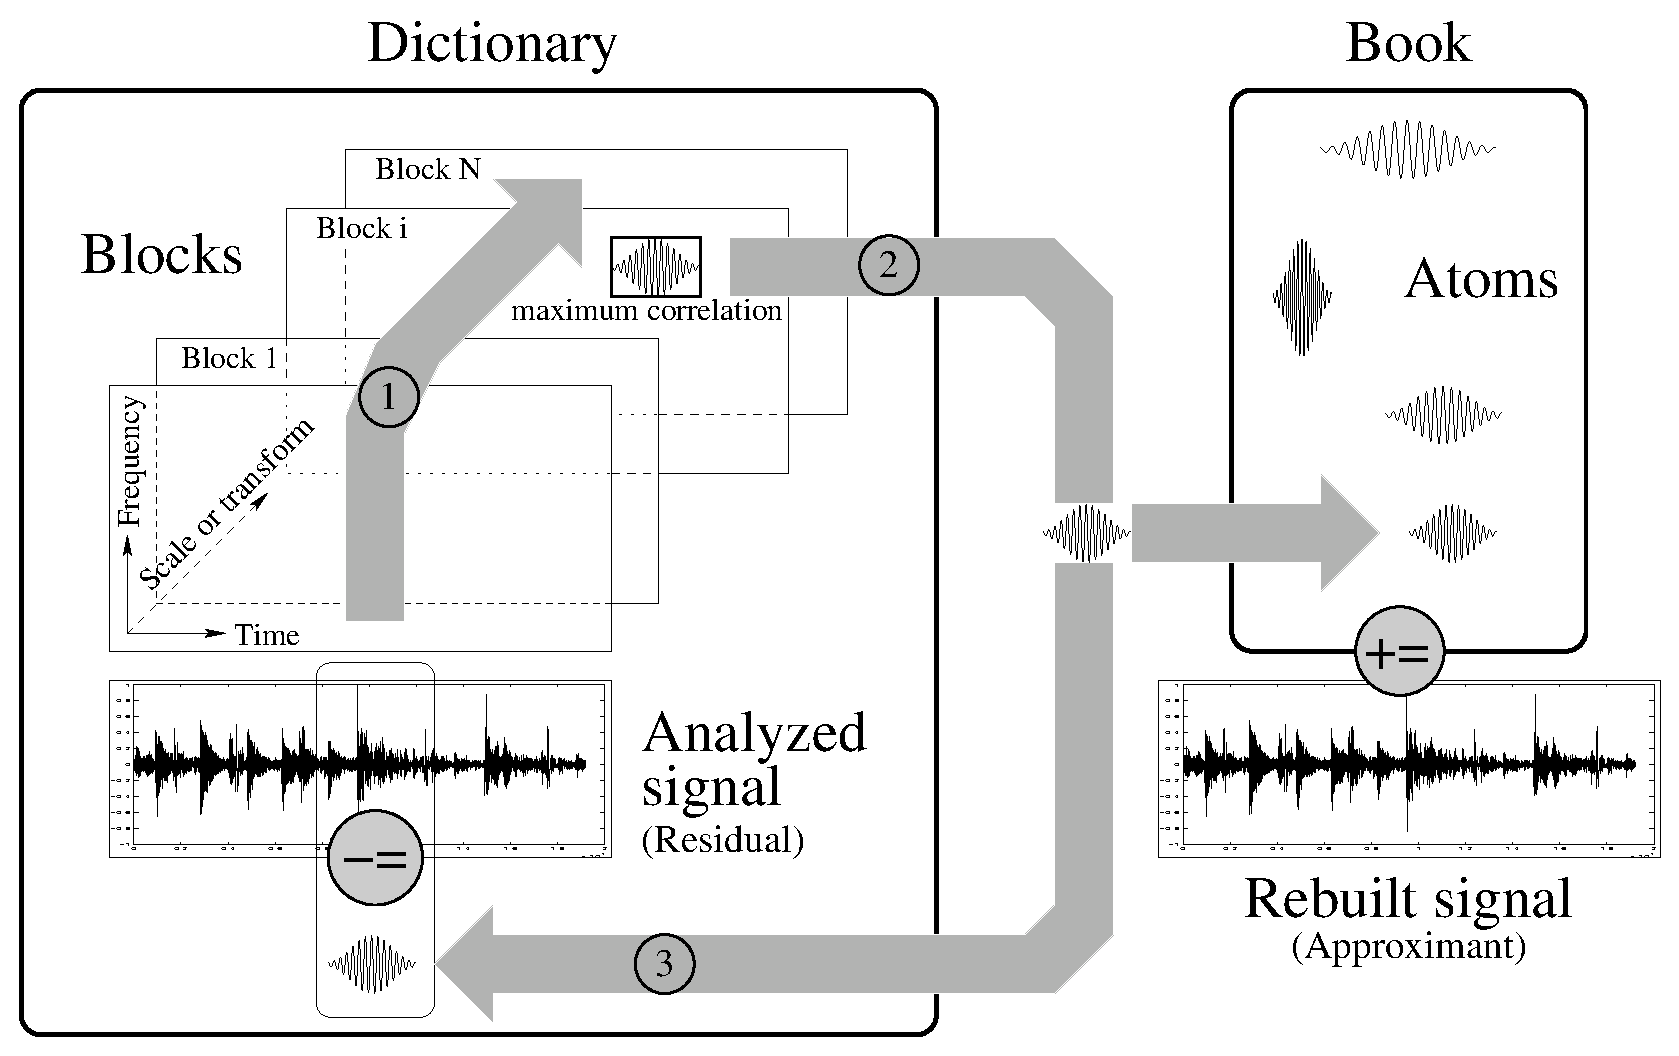
\includegraphics[width = 15cm, height=9cm]{Images/mpcycle.eps}
	\textit{\caption{\label{mpcycle} Description of Matching Pursuit. (See sections~\ref{term}/\ref{algo} for more explanations)}}
\end{figure}

\clearpage

%--------------------------------------------------------------
%--------------------------------------------------------------
% Section 2 : Basic download & install from sources
%--------------------------------------------------------------
%--------------------------------------------------------------
\chapter{Basic download \& install from source \label{DownInstSources}}

%--------------------------------------------------------------
% Section 2.1 : Getting the sources
%--------------------------------------------------------------
\section{Getting the sources}

The MPTK sources archives can be found under the gforge website, where you will be able 
to download any version of MPTK (https://gforge.inria.fr/frs/?group\_id=36) :
\begin{my_itemize}	
	\item MPTK source archives : ``MPTK-Source-v.v.v.tar.gz'' (current version is \input{CommandUsage/MPTKVersion})
\end{my_itemize}

%--------------------------------------------------------------
% Section 2.2 : Basic installation under Windows
%--------------------------------------------------------------
\section{Basic installation under Windows}

% Section 2.2.1 : Required tools

\subsection{Required tools}
\begin{my_itemize}
	\item \underline{Necessary :}
	\begin{my_itemize}
		\item Cmake (tested with version 2.8.3)\\
		\emph{$\mapsto$ To obtain it : http://www.cmake.org/cmake/resources/software.html}
		\item Microsoft Visual Studio (tested with free Visual C++ 2008 Express)\\
		\emph{$\mapsto$ To obtain it : http://www.microsoft.com/express}
	\end{my_itemize}
	\item \underline{Optional (if Matlab is needed) :}
	\begin{my_itemize}
		\item Matlab at least version R2006, \textbf{preferably} installed in the default directory :
		\begin{my_itemize}
			\item C:\textbackslash Program Files\textbackslash MATLAB
		\end{my_itemize}
	\end{my_itemize}
\end{my_itemize}

If the required tools are installed as mentioned, you should be able to generate 
a build system using the basic build settings.

% Section 2.2.3 : Pre-configuration using cmake

\subsection{Pre-configuration using cmake}

Suppose you unzip MPTK-Source-v.v.v.tar.gz in directory c:\textbackslash foo and you want to build MPTK 
files in c:\textbackslash bar (you may choose to build in a temporary location which differ 
from the place where you will eventually install MPTK). Use CMake to generate the build 
system, use the Make icons from the program menu to launch the CMake configuration application :

\begin{figure}[H]
	\centering
	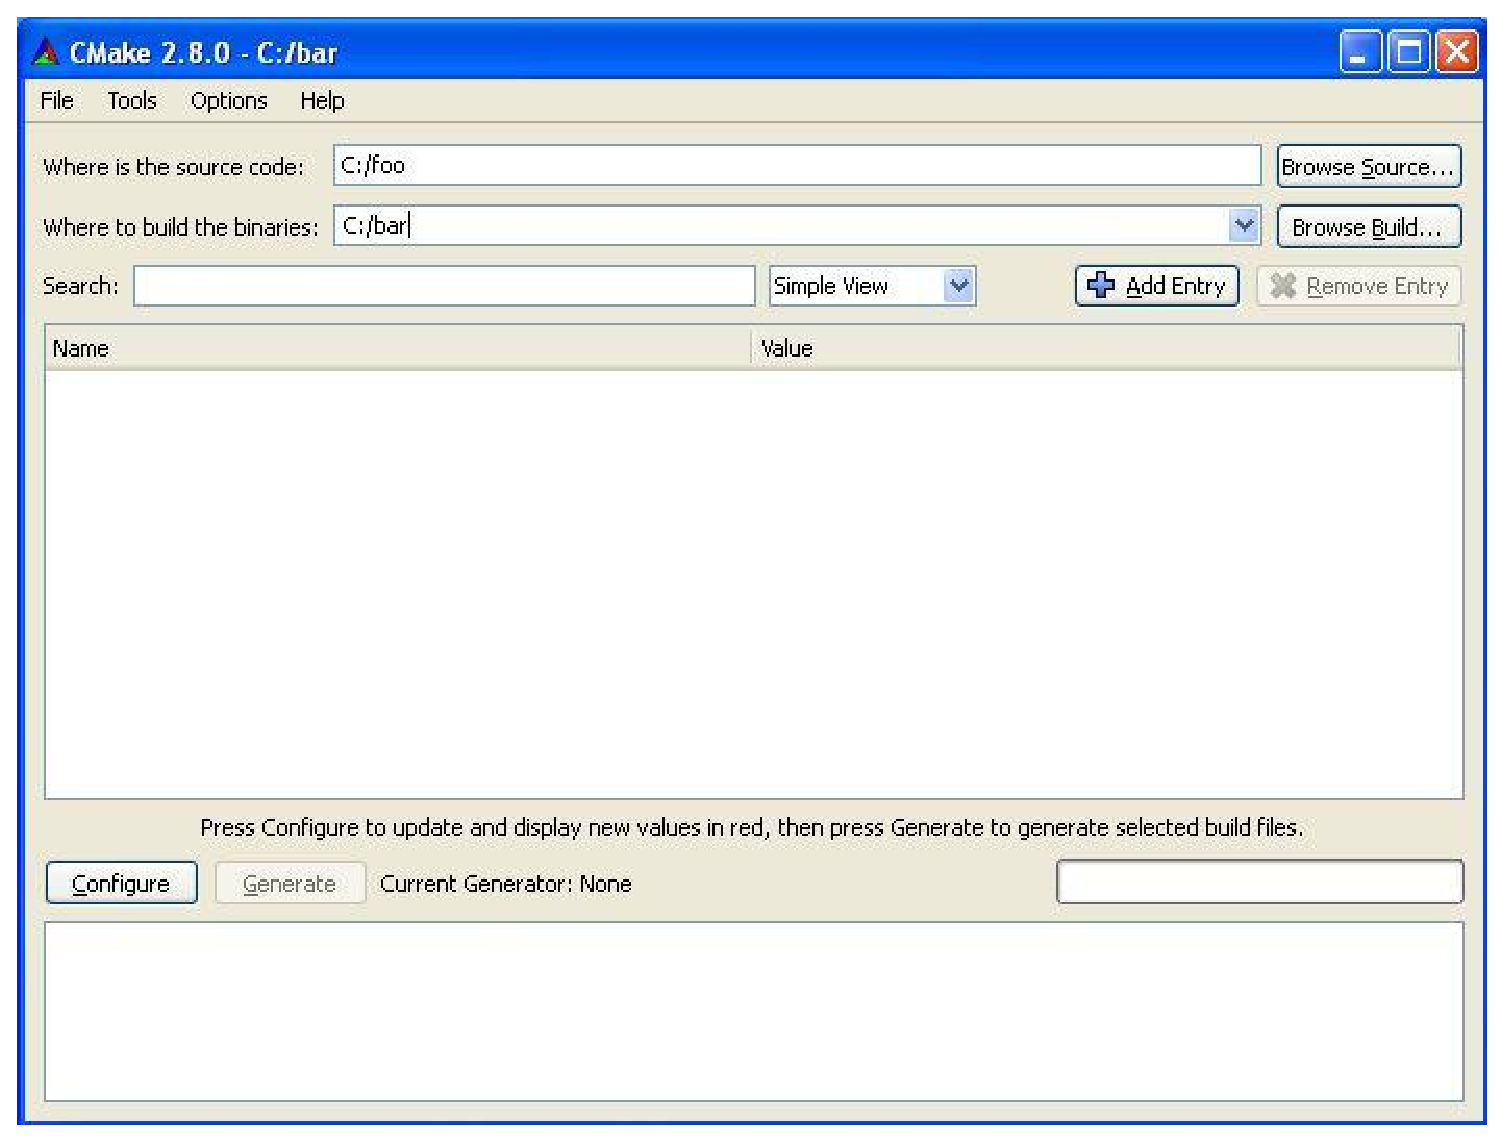
\includegraphics[width = 7cm, height=4cm]{Images/WindowsCmake.eps}
	\textit{\caption{\label{WindowsCmake} Cmake view under windows}}
\end{figure}

Set the ``Where is the source code'' text box with the path of the directory where the source files are 
located (c:\textbackslash foo) and the ``Where to build the binaries'' with the path of the directory 
where you want to build the library and executable files (c:\textbackslash bar).

When clicking for the first time on the [Configure] button, CMake will ask for the build tool you want to use. 
The build system type depends on the builder you want to use, in our case this is the Visual Studio 9 chain tools :

\begin{figure}[H]
	\centering
	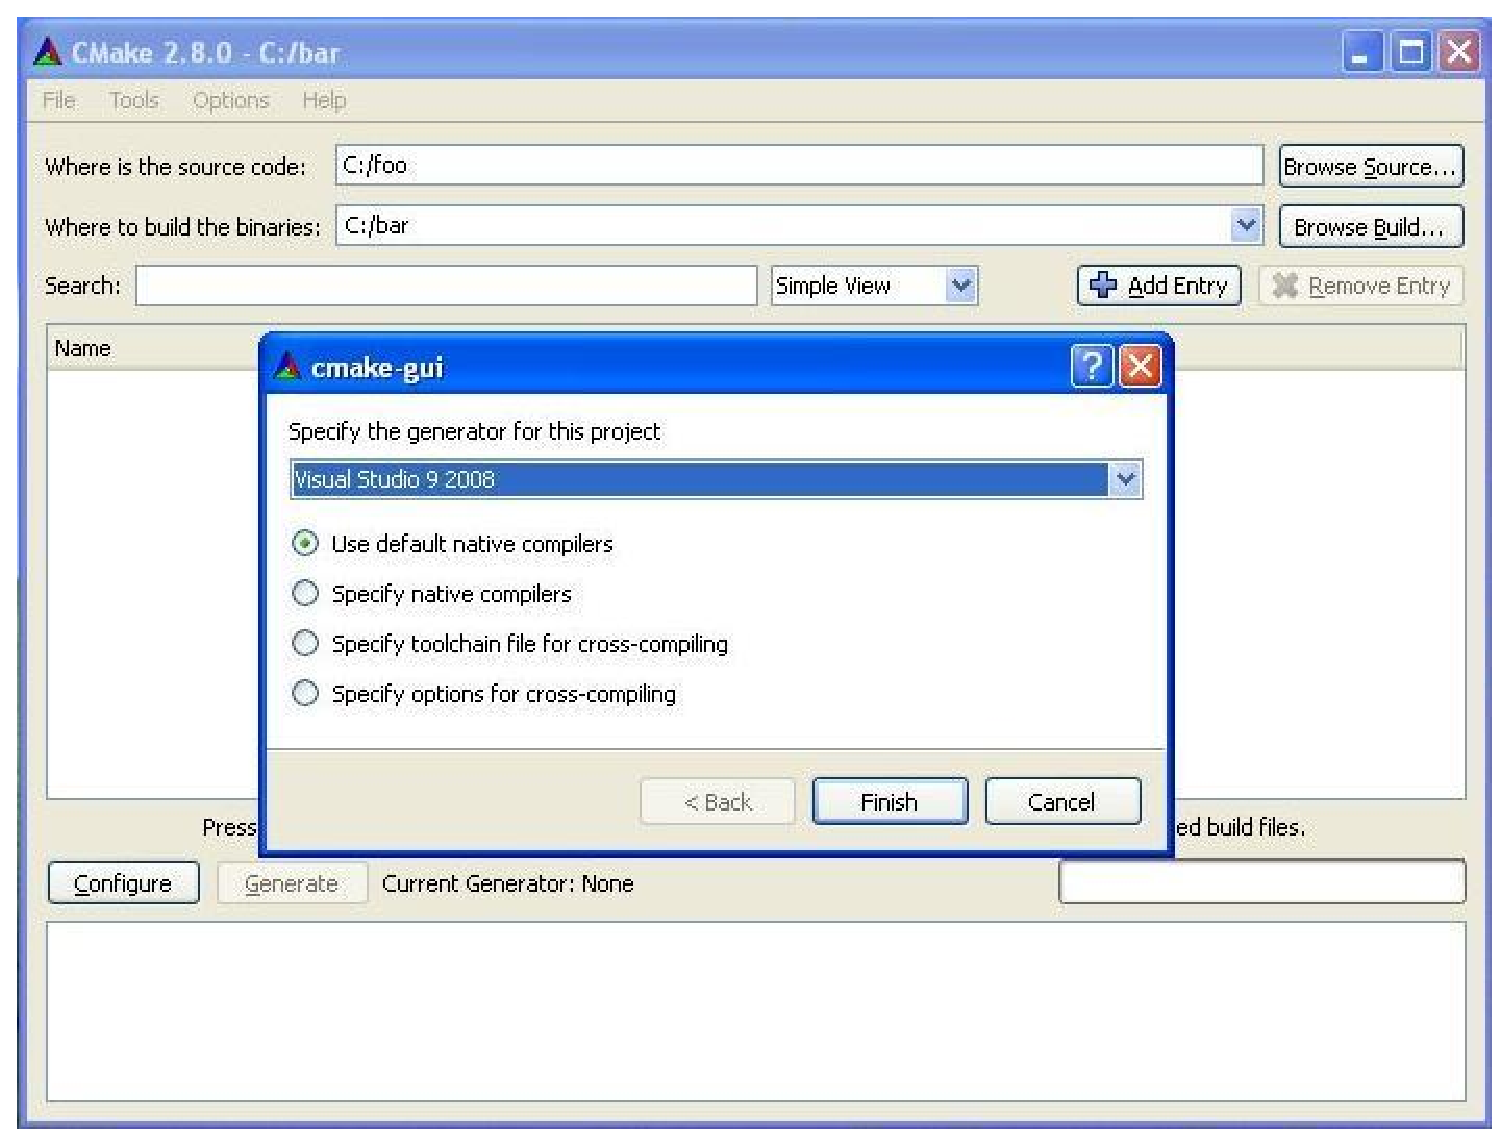
\includegraphics[width = 7cm, height=4cm]{Images/VisualStudioCmake.eps}
	\textit{\caption{\label{VisualStudioCmake} Cmake configuration using Visual Studio}}
\end{figure}

When pressing again the [Configure] button to configure the build system, CMake performs a list of tests 
to determine the system configuration and manage the build system. If the configuration is correct then no 
pop-up will appears during the tests and CMake finally shows the various options of the build underlaid in grey. 
In case of a configuration issue, a pop up window warns you about this issue indicating which test has failed, 
in this case the build option in the CMake application software will be underlaid in red. We will discuss in 
section~\ref{install_trouble} ``Installation Troubleshooting'' what to do in such a case, but let us for the moment assume that 
everything ran smoothly.

\vspace{0,7 cm}

Once the build system is configured then generated, you have to build MPTK using Visual.

\begin{figure}[H]
	\centering
	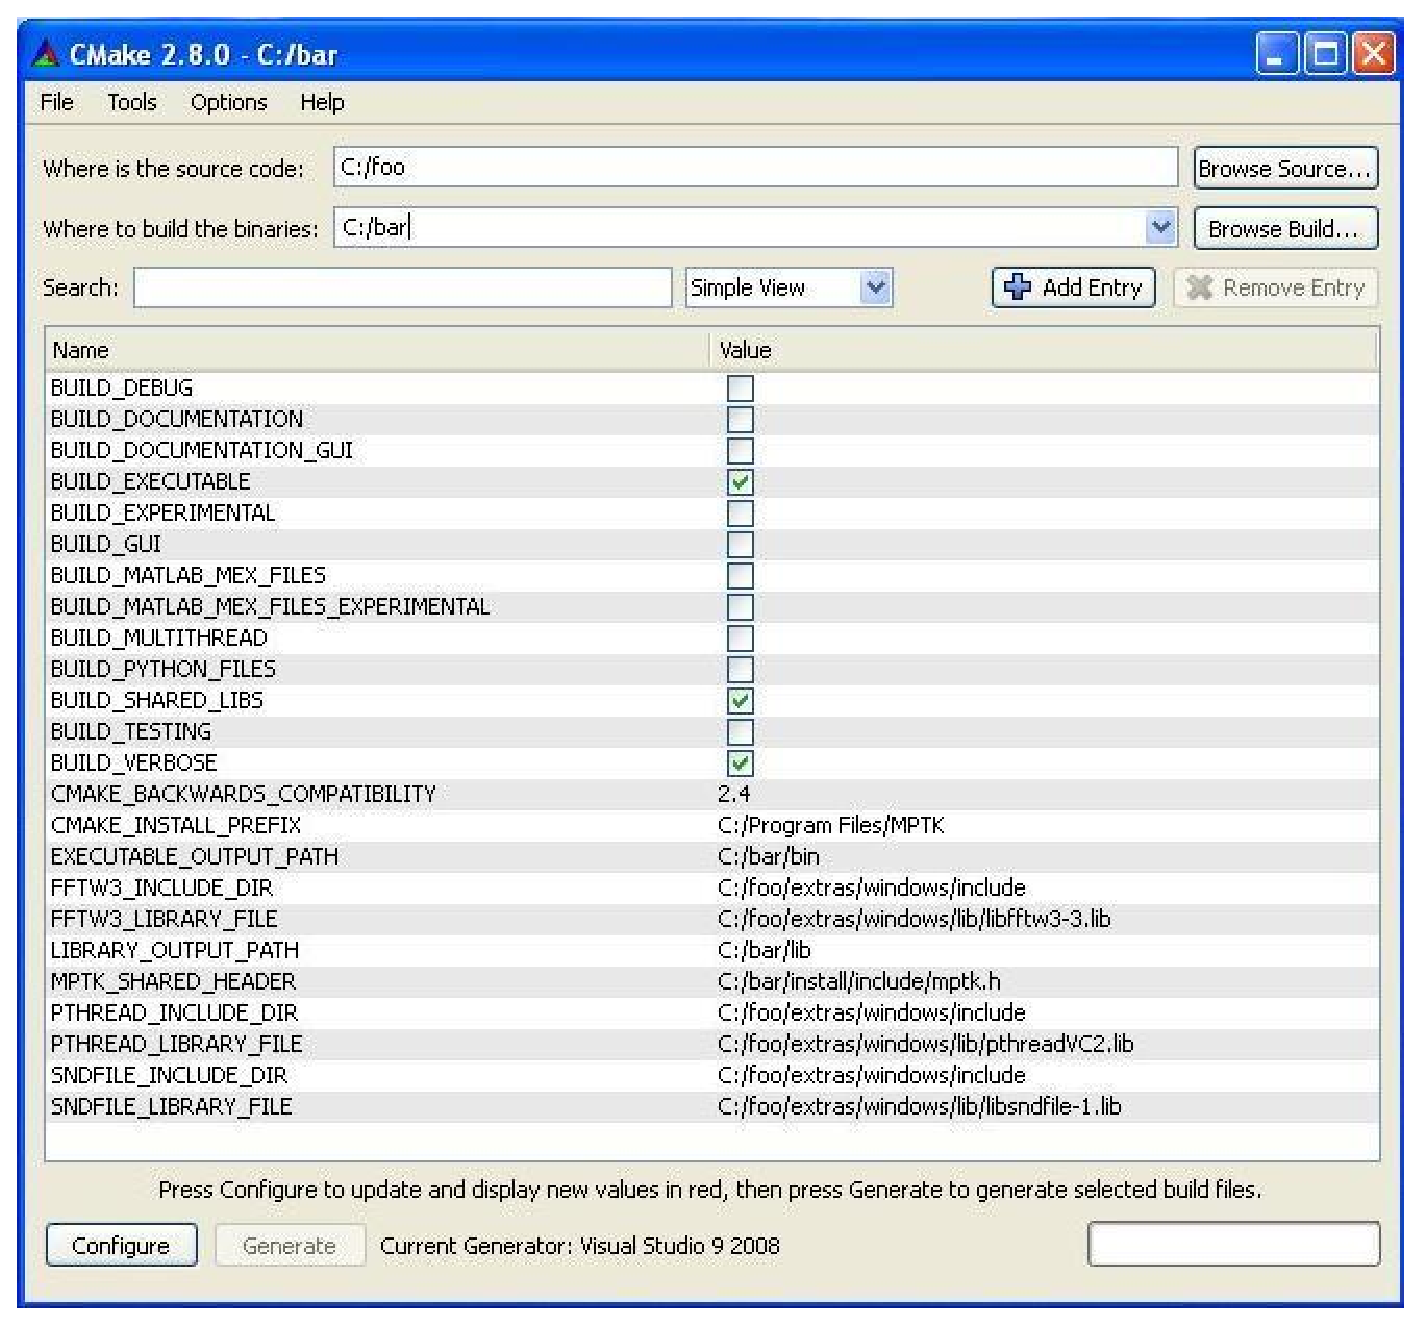
\includegraphics[width = 7cm, height=4cm]{Images/WindowsCmake2.eps}
	\textit{\caption{\label{WindowsCmake2} Cmake build system view for MPTK}}
\end{figure}

% Section 2.2.4 : Basic build

\subsection{Basic build}
Once the project is generated using Cmake, the build directory (ex : C:/bar)  contains a Visual solution 
(MPTK.sln).  When you double click on this file, Visual Studio software starts and opens the differents 
projects associated with this solution.

Right clicking on the project ``ALL\_BUILD'' located on the left tab of Visual Studio, then selecting 
``Generate'' will compile all the MPTK binary files.

% Section 2.2.5 : Basic installation

\subsection{Basic installation}
Right clicking on the project �``INSTALL'' located on the left tab of Visual Studio, then selecting
``This Project'' $\mapsto$ ``Generate only INSTALL'' will install MPTK to the directory associated with
 the ``MPTK\_INSTALL\_PREFIX'' variable of Cmake.
 
 
%--------------------------------------------------------------
% Section 2.3 : Basic installation under Unix & MacOS
%--------------------------------------------------------------
\section{Basic installation under Unix \& MacOS}
If the required libraries are installed as the appendix \ref{GetLibsndfile} and \ref{GetFftw} indicate it, you should be able 
to generate a build system using the basic build settings.

% Section 2.3.1 : Required tools

\subsection{Required tools}
\begin{my_itemize}
	\item \underline{Necessary :}
	\begin{my_itemize}
		\item Cmake (tested with version 2.8.3)\\
		\emph{$\mapsto$ To obtain it : http://www.cmake.org/cmake/resources/software.html}
	\end{my_itemize}
	\item \underline{Optional (if Matlab is needed) :}
	\begin{my_itemize}
		\item Matlab at least version R2006, \textbf{Preferably} installed in the default directory :
		\begin{my_itemize}
			\item For Linux : /opt/MATLAB\_Ryyyyx or /soft/MATLAB\_Ryyyyx
			\item For Mac : /Applications/MATLAB\_Ryyyyx (with yyyy = year, x=[a-z])
		\end{my_itemize}
	\end{my_itemize}
\end{my_itemize}

% Section 2.3.2 : Required packages

\subsection{Required packages}

\begin{my_itemize}
	\item Libsndfile pre-compiled library (tested with version 1.0.21) 
	\item FFTW pre-compiled library (tested with version 3.2.2)
\end{my_itemize}

% Section 2.3.3 : Pre-configuration using cmake

\subsection{Pre-configuration using cmake}
Suppose you untar ``MPTK-Source-v.v.v.tar.gz'' in directory \verb+~+/foo and you want to build MPTK binary 
and library files in \verb+~+/bar.

The Command list you should use will look like this : \newline
\begin{tt}
    	bash-3.1\$ mkdir \verb+~+/bar \newline
	bash-3.1\$ cd \verb+~+/bar \newline
	bash-3.1\$ cmake \verb+~+/foo \newline
\end{tt}
	
When using the cmake command to generate the build system, Cmake performs a list of tests to 
determine the system configuration and manage the build system. If the configuration is correct 
then the build system is generated and written. In this case the three last lines of the console log 
of cmake command should be: \newline
\begin{tt}
	... \newline
	bash-3.1\$ -- Configuring done \newline
	bash-3.1\$ -- Generating done \newline
	bash-3.1\$ -- Build files have been written to: \verb+~+/bar
\end{tt}

% Section 2.3.4 : Basic build

\subsection{Basic build}
The command {\tt make} will compile the build files and should finish like : \newline
\begin{tt}
	... \newline
	bash-3.1\$ Linking CXX executable ../../bin/test\_windowLen \newline
	bash-3.1\$ [100\%] Built target test\_windowLen \newline
\end{tt}

% Section 2.3.5 : Basic installation

\subsection{Basic installation}
The command {\tt sudo make install} will install in default directory ``path\_to\_MPTK`` and should finish like this : \newline
\begin{tt}
	... \newline
	bash-3.1\$ -- Installing: /usr/local/lib/liblibmd5sum.a \newline
	bash-3.1\$ -- Installing: /usr/local/lib/liblibgetopt.a \newline
\end{tt}
Or like this if the documentation has been generated using the option BUILD\_DOCUMENTATION of CMake :
\begin{tt}
	... \newline
	bash-3.1\$ -- Installing: /usr/local/lib/liblibmd5sum.a \newline
	bash-3.1\$ -- Installing: /usr/local/lib/liblibgetopt.a \newline
	bash-3.1\$ -- Installing: /usr/local/doc/short\_description.pdf \newline
	bash-3.1\$ -- Installing: /usr/local/doc/GettingStarted.pdf \newline
	bash-3.1\$ -- Installing: /usr/local/doc/userman.pdf \newline
\end{tt}

%--------------------------------------------------------------
%--------------------------------------------------------------
% Section 3 : CMake options & troubleshooting
%--------------------------------------------------------------
%--------------------------------------------------------------
\chapter{CMake options \& troubleshoot \label{CMakeTrouble}}

%--------------------------------------------------------------
% Section 3.1 : Using ccmake to set build options
%--------------------------------------------------------------
\section{Using ccmake to set build options}
The Cmake Graphical User Interface is automaticaly displayed under Windows OS, and is available with 
the command {\tt ccmake} under Unix OS. It allows you to :
\begin{my_itemize}
	\item Specify build system options, such as either to enable the use of multiple threads to speed 
		up the Matching Pursuit decomposition or to generate the doxygen documentation
	\item Troubleshoot the various paths required to build MPTK
	\item Display advanced build options via the advanced mode
\end{my_itemize}

\begin{figure}[H]
	\begin{minipage}[t]{.4\linewidth}
	 	\begin{center}
			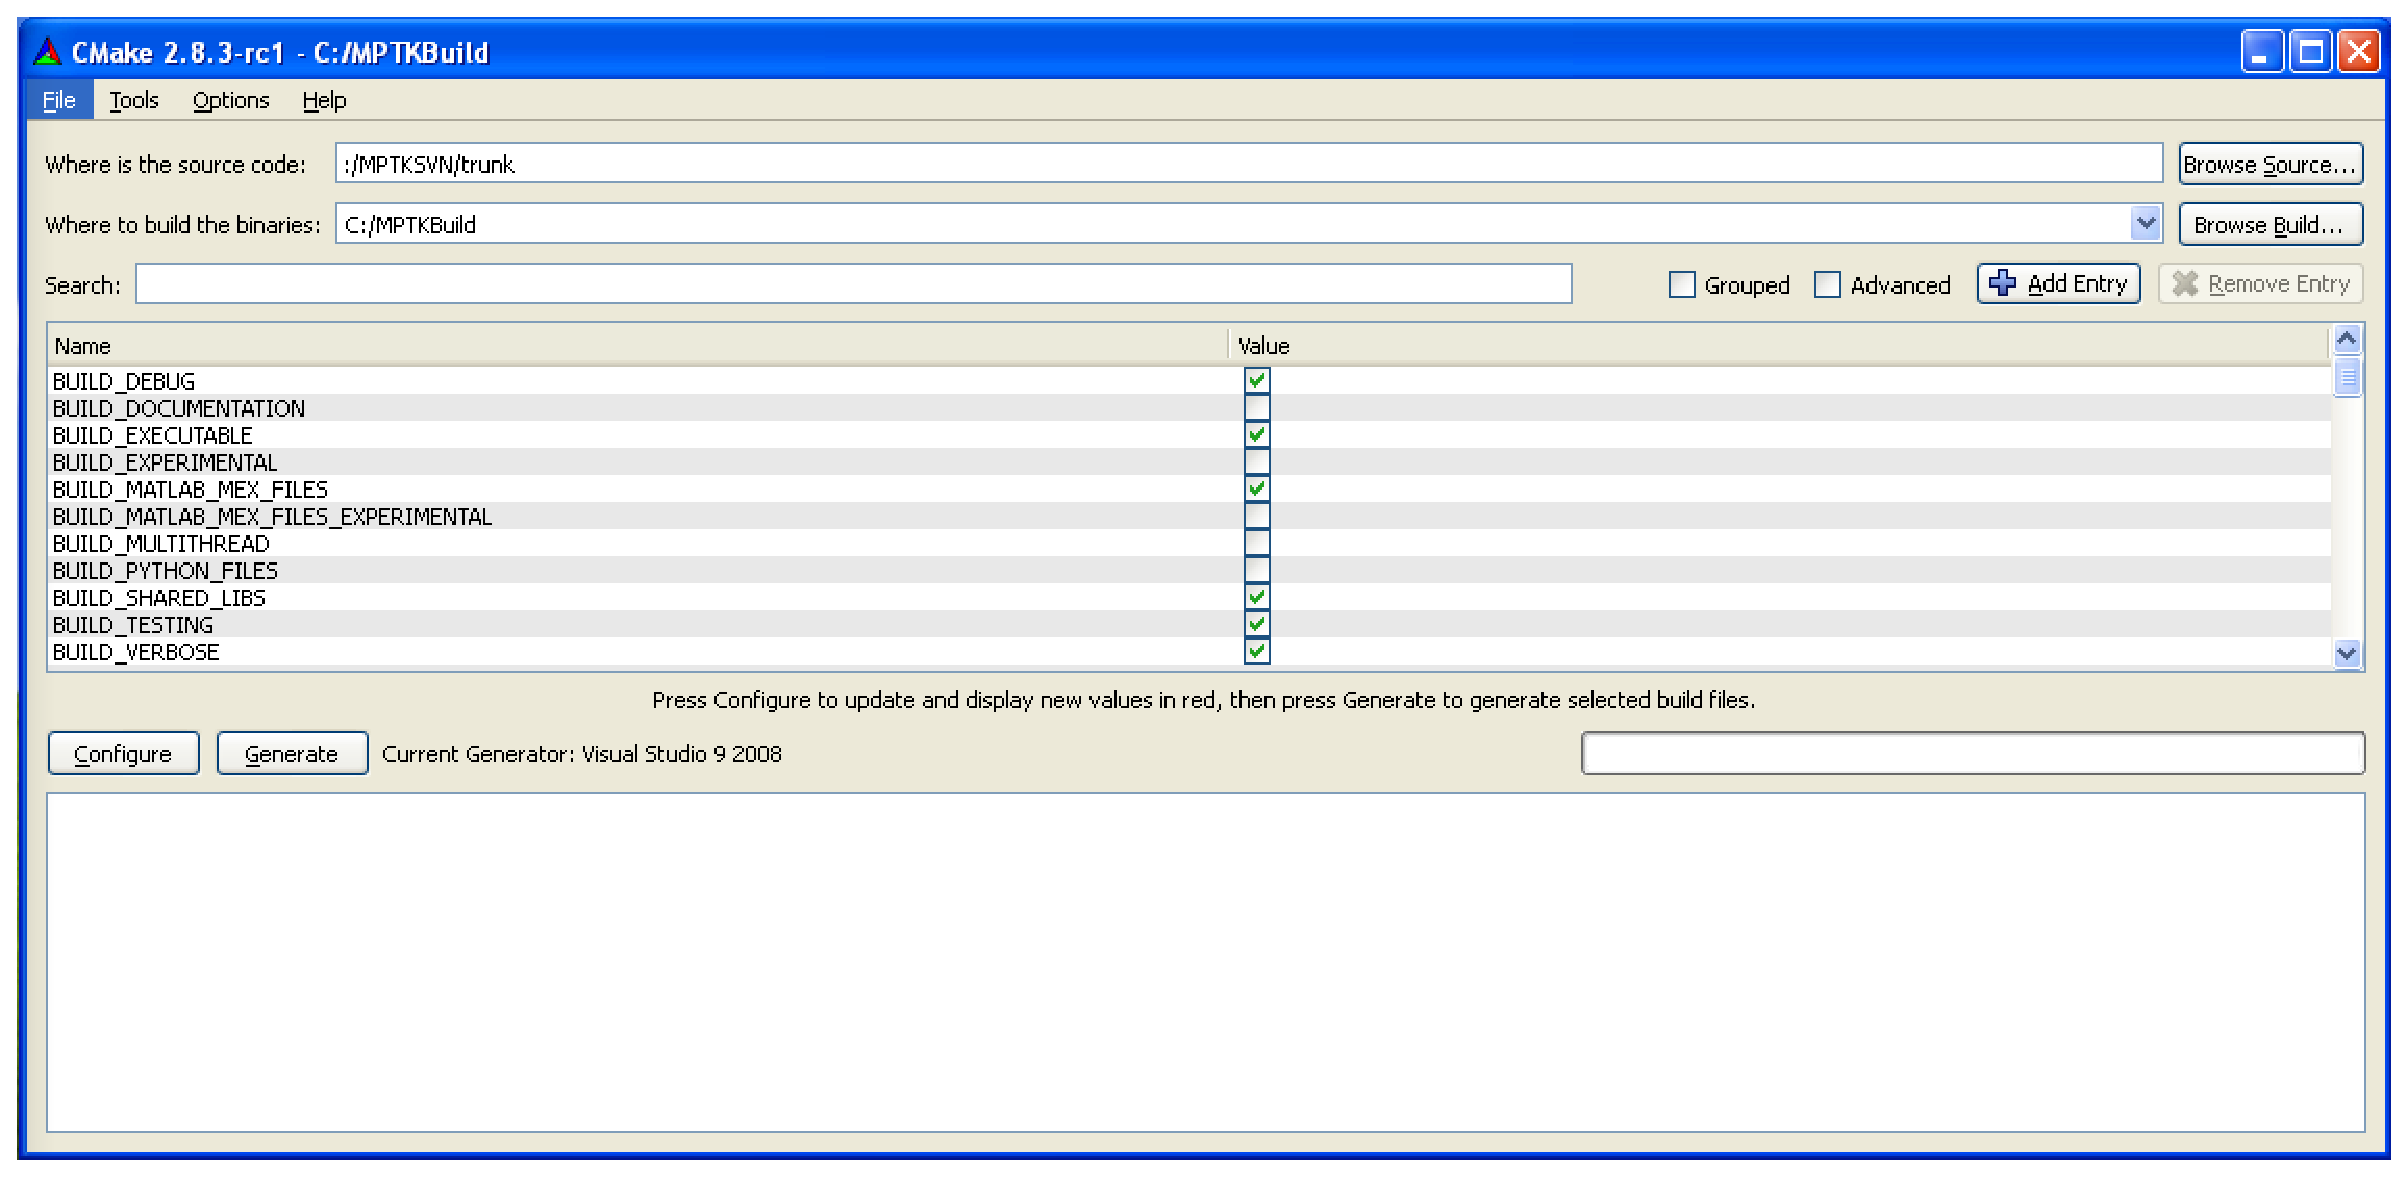
\includegraphics[width = 7cm, height=5cm]{Images/WindowsCMakeGUI.eps}
			\textit{\caption{\label{WindowsCMakeGUI} Windows CMake GUI}}
		\end{center}
	\end{minipage}
	\hfill
	\begin{minipage}[t]{.4\linewidth}
		\begin{center}
			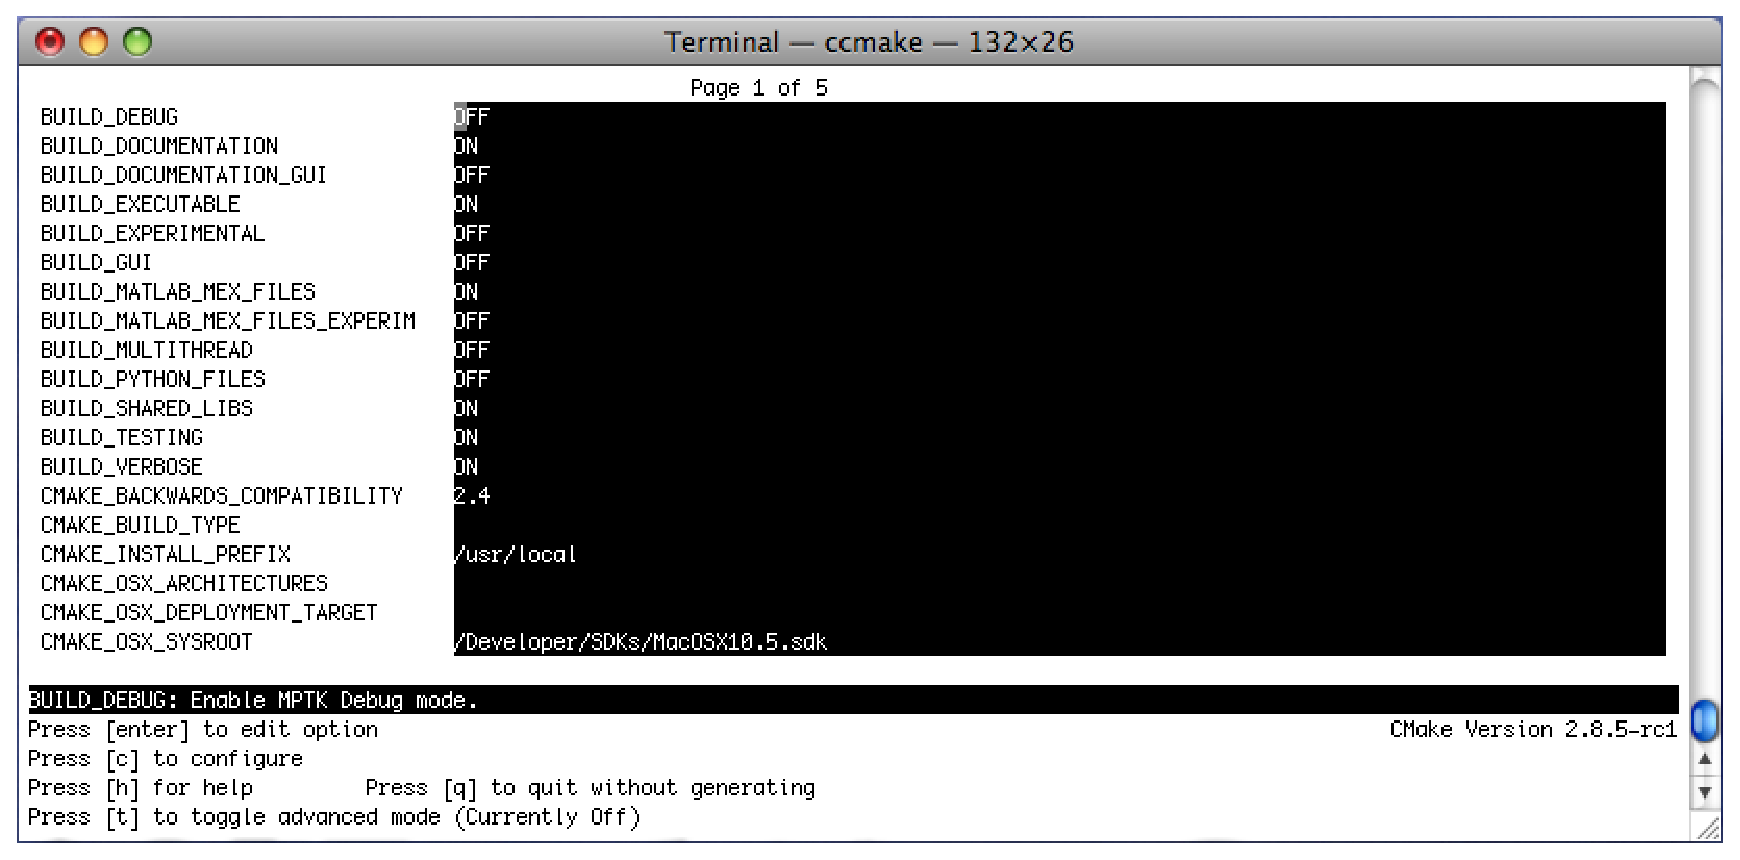
\includegraphics[width = 7cm, height=5cm]{Images/UnixCMakeGUI.eps}
			\textit{\caption{\label{UnixCMakeGUI} Unix CMake GUI}}
		\end{center}
	\end{minipage}
\end{figure}

%--------------------------------------------------------------
% Section 3.2 : Main options 
%--------------------------------------------------------------
\section{Main options}
This Graphical User Interface allows the user to set the build options for MPTK :
\begin{my_itemize}
	\item CMAKE\_INSTALL\_PREFIX : Path of the installation (by default: /usr/local/)
	\item BUILD\_DOCUMENTATION : Generation of the doxygen documentation library. 
		This operation can take a lot of time, be patient. (by default : OFF)
	\item BUILD\_DOCUMENTATION\_GUI : Generation of the doxygen documentation for 
		the Graphical User Interface. Careful, it can take a lot of time. (by default : OFF)
	\item MULTITHREAD : Allow MPTK to use parrallel computing, this option allows to 
		increase performance on multi-processor hardware architectures (by default : OFF)
\end{my_itemize}

\clearpage

%--------------------------------------------------------------
% Section 3.3 : Advanced options
%--------------------------------------------------------------
\section{Advanced options}
You can display more information and all the configuration options by switching to the advanced mode, 
which is set to off by defaut and can be toggled on by pressing [t].

\vspace{0,3 cm}

\noindent The list of the following options should be considered as advanced:
\begin{my_itemize}
	\item BUILD\_DEBUG : Compile in debug mode (by default: OFF = Release)
	\item BUILD\_SHARED\_LIBS: Allows the construction of libraries (libdsp\_windows \& libmptk) 
	in a lib directory and the include file (mptk.h) in an include directory (by default: ON)
	\item BUILD\_TESTING: Allow to test executables using Dart server (by default : ON)
	\item BUILD\_VERBOSE: Display various informations during the build (by default : ON)
	\item BUILD\_EXECUTABLE: Build the executables mpd, mpf...  (by default: ON)
\end{my_itemize}

%--------------------------------------------------------------
% Section 3.4 : Troubleshooting build issues
%--------------------------------------------------------------
\section{Troubleshooting build issues \label{install_trouble}}


% Section 3.4.1 : Installation troubleshoot

\subsection{CMake GUI issues}
Let's see a more complex use of the Cmake GUI troubleshooting. Despite all the integrated 
tests when Cmake manages to generate the build system of MPTK, sometimes Cmake cannot 
determine some parameters of your configuration. When using the cmake command, Cmake 
performs a list of tests on the build system configuration in order to generate it, if there is some 
issue related to the configuration, the errors list is displayed at the end of the consol log. Here 
we have 4 includes files or libraries that Cmake cannot found :

\begin{figure}[H]
	\centering
	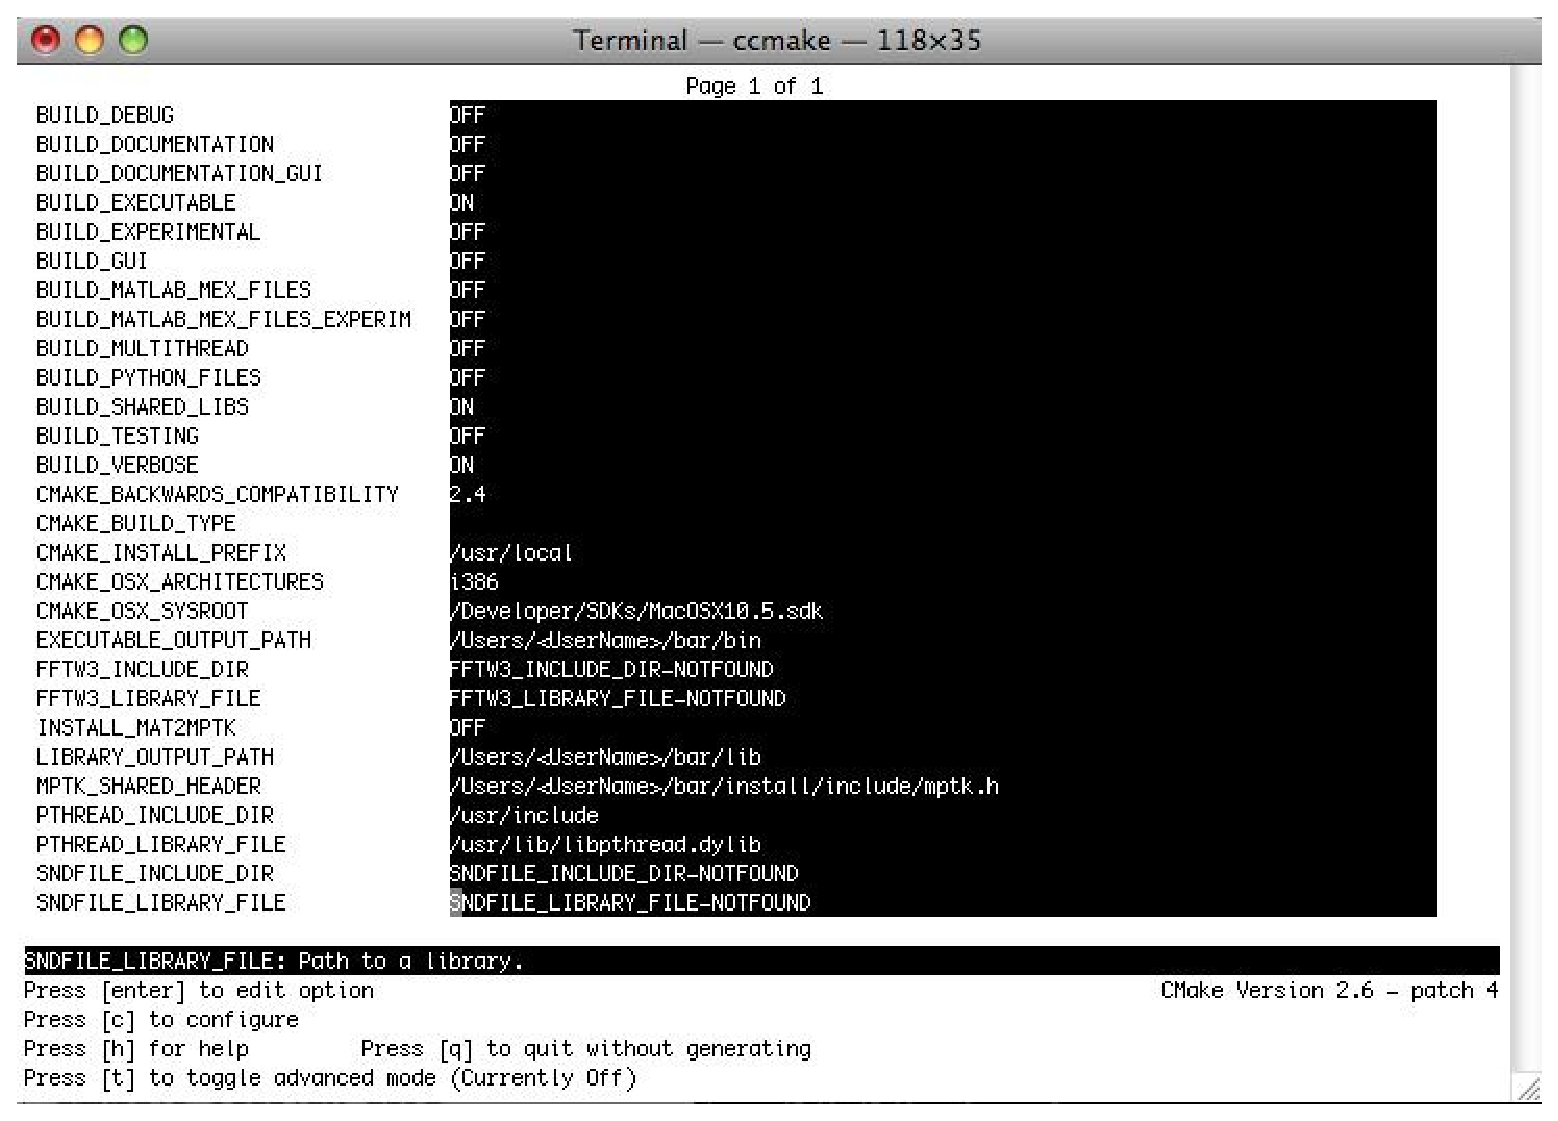
\includegraphics[width = 7cm, height=4cm]{Images/FailedCmake.eps}
	\textit{\caption{\label{FailedCmake} Example view of cmake libraries detection failed}}
\end{figure}

In this current case, {\tt FFTW3\_INCLUDE\_DIR}, {\tt FFTW3\_LIBRARY\_FILE}, {\tt SNDFILE\_INCLUDE\_DIR} 
and {\tt SND\_LIBRARY\_FILE} fields must be set with the path to the directory containing 
the FFTW and sndfile libraries. To set the fields values simply press [enter] while the cursor is on the 
relevant field, and after editing press [enter] to escape the field edition.  

\vspace{0,3 cm}

\noindent \underline{Important note:} In the case of  include files, only the directory where this include files are located 
is required. But in the case of library files, the entire path to the library including its name must be indicated 
in the corresponding field.

\vspace{0,3 cm}

After choosing the options for the build and setting the required fields, press [c] to configure. The configuration 
of the build system is checked again by Cmake, at the end of this check if the build settings are correct, you 
can press [g] in order to generate the build system and quit the Cmake GUI.



% Section 3.4.2 : Fixing FFTW used plan with wisdom in FFTW configuration

\subsection{Fixing FFTW used plan with wisdom in FFTW configuration}
MPTK currently relies on FFTW to compute Fast Fourier Transforms. The principle of FFTW is to 
adaptively select the fastest running codelet to perform a given FFT, which is good for performance. 
However, this can lead to non deterministic behaviour of MPTK since two consecutive runs of the 
same command (e.g. `mpd') with the same options on the same data can yield slightly different results. 
To avoid this issue we have implemented a mechanism which allows MPTK to fix which FFT codelet 
is used for a specific type of FFT computation. To do this, you just need to create and export a 
environment variable called MPTK\_FFTW\_WISDOM and set this environnement variable with 
the path of the file you want to use in order to save the FFTW configuration. MPTK will create 
a ``wisdom'' file, that will be reloaded each time you use MPTK. It means that the codelets use 
to compute FFTW plan will be the same between two successive decompositions with the same parameters.

\vspace{0,3 cm}

\noindent For bash or sh or ash:

\vspace{0,2 cm}

\noindent {\tt bash-3.1\$ export MPTK\_FFTW\_WISDOM=/usr/local/fftw\_wisdom\_file}

\vspace{0,3 cm}

If you want to fix permanently the used FFTW plan, just set this environment variable when the console 
is launched, using for that the /etc/profile, ~/.profile or  .bashrc file, according to your system configuration. 

\vspace{0,3 cm}

\noindent For tcsh or csh : 

\vspace{0,2 cm}

\noindent {\tt bash-3.1\$ setenv MPTK\_FFTW\_WISDOM=/usr/local/fftw\_wisdom\_file}

\vspace{0,3 cm}

If you want to fix permanently the used FFTW plan, just set this environment variable when the console 
is launched, using for that the  /etc/csh.cshrc file, according to your system configuration.

\clearpage

%--------------------------------------------------------------
%--------------------------------------------------------------
% Section 3 : How to use MPTK command lines
%--------------------------------------------------------------
%--------------------------------------------------------------
\chapter{How to use MPTK command lines \label{UseCmdLine}}

%--------------------------------------------------------------
% Section 3.1 : Beginning with command lines
%--------------------------------------------------------------
\section{Beginning with command lines}

\noindent \underline{Unix \& MacOS: }

\vspace{0,2 cm}

The installation is supposed to copy the binary files (mpd, mpr, mpf...) 
under ``/usr/local/bin'' and the library files under ``/usr/local/lib'' which are supposed to be under the 
environment PATH destination. You should normaly be able to launch it directly using terminal command. 

\vspace{0,2 cm}

Try typing ``mpd'' under a terminal command and then you should see the help description.

\vspace{0,3 cm}

\noindent \underline{Windows: }

\vspace{0,2 cm}

The installation is supposed to copy the binary files (mpd, mpr, mpf...) and the library files 
under ``C:\textbackslash Program Files\textbackslash MPTK\textbackslash bin''. In order to make it work, type 
``cmd'' under the execute launcher. Then try typing ``C:\textbackslash Program Files\textbackslash 
MPTK\textbackslash bin\textbackslash mpd.exe'' and then you should see the help description.

%--------------------------------------------------------------
% Section 3.2 : Introduction
%--------------------------------------------------------------
\section{Introduction}

The Matching Pursuit standalone utilities are designed so that a typical
processing task decomposes into a chain of commands which can be connected by
pipes. The signal decomposition is performed by {\tt mpd}. The atoms stored in
the resulting books can be filtered (i.e., sorted and selected) with the
command {\tt mpf}. Several books can then be concatenated with the command {\tt
  mpcat}. Once a desired book is obtained, a corresponding approximant signal
can be rebuilt using {\tt mpr}, with the optional addition of a residual signal
(or in addition to any other signal). Alternately, the {\tt mpd\_demix} utility
provides blind source separation using Matching Pursuit when the mixing matrix
is known. Each of the cited utilities have a {\tt -h} switch to get
command-line help.

\smallskip

\noindent Some typical processing chains include:

\begin{itemize}
\item Signal approximation with N atoms: \\
      \mbox{\tt mpd -D dictionary -n N soundFile.wav book.bin;} \\
      \mbox{\tt mpr book.bin approx.wav} \\
      -- or -- \\
      \mbox{\tt mpd -D dictionary -n N soundFile.wav - | mpr - approx.wav}
\item Exact reconstruction: \\
      \mbox{\tt mpd -D dictionary -n N soundFile.wav book.bin residual.wav;} \\
      \mbox{\tt mpr book.bin approx.wav residual.wav}
\item Signal approximation, using only the short atoms (e.g., of less than
128~samples) \linebreak and ignoring the residual: \\
      \mbox{\tt mpd -D dictionary -n N soundFile.wav book.bin;} \\
      \mbox{\tt mpf --length=[0:128] book.bin bookShort.bin;} \\
      \mbox{\tt mpr bookShort.bin approx.wav}
\item Blind source separation and rebuilding an approximation of one of the
  sources (e.g., the~3rd one): \\
      \mbox{\tt mpd\_demix -D dictionary -M matrix.txt -n N mix.wav bookFile;} \\
      \mbox{\tt mpr bookFile\_3.bin approxOfSource3.wav}
\end{itemize}

Lots of other combinations are possible. The relevant utilities are described
with more detail in the next sections.

\vspace{0,3 cm}

\textbf{\emph{Note about the signal file formats:}} MPTK has been originally designed for sound
processing, but it is applicable to any kind of signal.

For input, we have mostly been using the WAV format, but any ``fees free'' file format
recognized by the \texttt{libsndfile} library (OGG, AIFF, FLAC...) should work with 
the provided MPTK utilities. MP3 is not supported for one very good reason, doing so requires 
the payment of licensing fees.

The signal output is more specific: the MPTK binaries output signals in the WAV
format only. {\em (WARNING: in the \texttt{libsndfile} implementation, this 
format is not protected against clipping, which may happen for some books and 
is not an artifact of the MPTK analysis.)} Nevertheless, the MPTK API also
offers Matlab, raw \verb+double+ and raw \verb+float+ signal output formats:
those could be quickly enabled by simple hacks of the relevant utilities. To
enable other output formats, please contribute some code to the
\verb+mp_signal.{h,cpp}+ API.

%--------------------------------------------------------------
% Section 3.3 : The MPTK environment
%--------------------------------------------------------------
\section{The MPTK environment}
In order to define the working environment of Matching Pursuit utilities, 
An XML file is loaded before using Matching Pursuit. This XML file contains
the configuration path \verb+<configpath>+ path\verb+</configpath>+ the syntax
of the path is \verb+<path name="NAME" path="PATH"/>+ the path used are:

\begin{itemize}
 \item \verb+dll_directory+ the directory where MPTK library search for plugins
                            Dynamic Link Library (DLL) defining atoms and blocks
 \item \verb+fftw_wisdomfile+ the default path for the FFTW wisdom file which allows
                              to save the setting for FFT computation.
\end{itemize}

This values can be set by two way, the complete path of the file can be specified
with the \verb+-C<FILE>, -config-file=<FILE>+ for utilities or MPTK library calls 
the environment variable \verb+MPTK_CONFIG_FILENAME+ to determine
which file to use for setting up the MPTK environment.

%--------------------------------------------------------------
%--------------------------------------------------------------
% Section 4 : List of command lines functions
%--------------------------------------------------------------
%--------------------------------------------------------------
\chapter{List of command lines functions \label{ListCmdLine}}

%--------------------------------------------------------------
% Section 4.1 : MPD
%--------------------------------------------------------------
\section{mpd: matching pursuit signal decomposition}
\input{CommandUsage/mpd_Usage}
\clearpage

%--------------------------------------------------------------
% Section 4.2 : GPD
%--------------------------------------------------------------
\section{gpd: gradient pursuit signal decomposition}
\input{CommandUsage/gpd_Usage}

%--------------------------------------------------------------
% Section 4.3 : MPR
%--------------------------------------------------------------
\section{mpr: signal reconstruction}
\input{CommandUsage/mpr_Usage}
\clearpage

%--------------------------------------------------------------
% Section 4.4 : MPF
%--------------------------------------------------------------
\section{mpf: filtering of the book files}
\input{CommandUsage/mpf_Usage}
\clearpage

%--------------------------------------------------------------
% Section 4.5 : MPCAT
%--------------------------------------------------------------
\section{mpcat: concatenation of book files}
\input{CommandUsage/mpcat_Usage}

%--------------------------------------------------------------
% Section 4.6 : MPD_DEMIX
%--------------------------------------------------------------
\section{mpd\_demix: blind source separation with a matrix}
\input{CommandUsage/mpd_demix_Usage}

%--------------------------------------------------------------
% Section 4.7 : MPVIEW
%--------------------------------------------------------------
\section{mpview: generation of a time-frequency map from a book}
\input{CommandUsage/mpview_Usage}
\clearpage

%--------------------------------------------------------------
%--------------------------------------------------------------
% Section 5: How to use MPTK with Matlab
%--------------------------------------------------------------
%--------------------------------------------------------------
\chapter{How to use MPTK with Matlab \label{UseMatlabFunc}}

%--------------------------------------------------------------
% Section 5.1 : Beginning with Matlab 
%--------------------------------------------------------------
\section{Beginning with Matlab}

Quoting Wikipedia ``MATLAB (MAtrix LABoratory) is a numerical computing environment. Developed by MathWorks, MATLAB 
allows matrix manipulations, plotting of functions and data, implementation of algorithms, creation of user interfaces, and 
interfacing with programs written in other languages, including C, C++, Java, and Fortran.''

\vspace{0,3 cm}

The one thing to understand when using Matlab is the path configuration. In fact, it works as a terminal : The available 
files are the ones present in the current selected path. When launching MATLAB, the default path is not the one required. 

% Section 5.1.1 : Temporary path configuration

\subsection{Temporary path configuration}

If the user wants to temporary change the path (in order to include MPTK path), there are three possibilities : 
\begin{my_itemize}
	\item Using the MATLAB native command ``addpath(path\_to\_MPTK/mptk/matlab)''
	\item Using the folder selection situated in the top of MATLAB window interface
	\item Using the terminal command ``cd path\_to\_MPTK/mptk/matlab''
\end{my_itemize}

\begin{figure}[H]
	\centering
	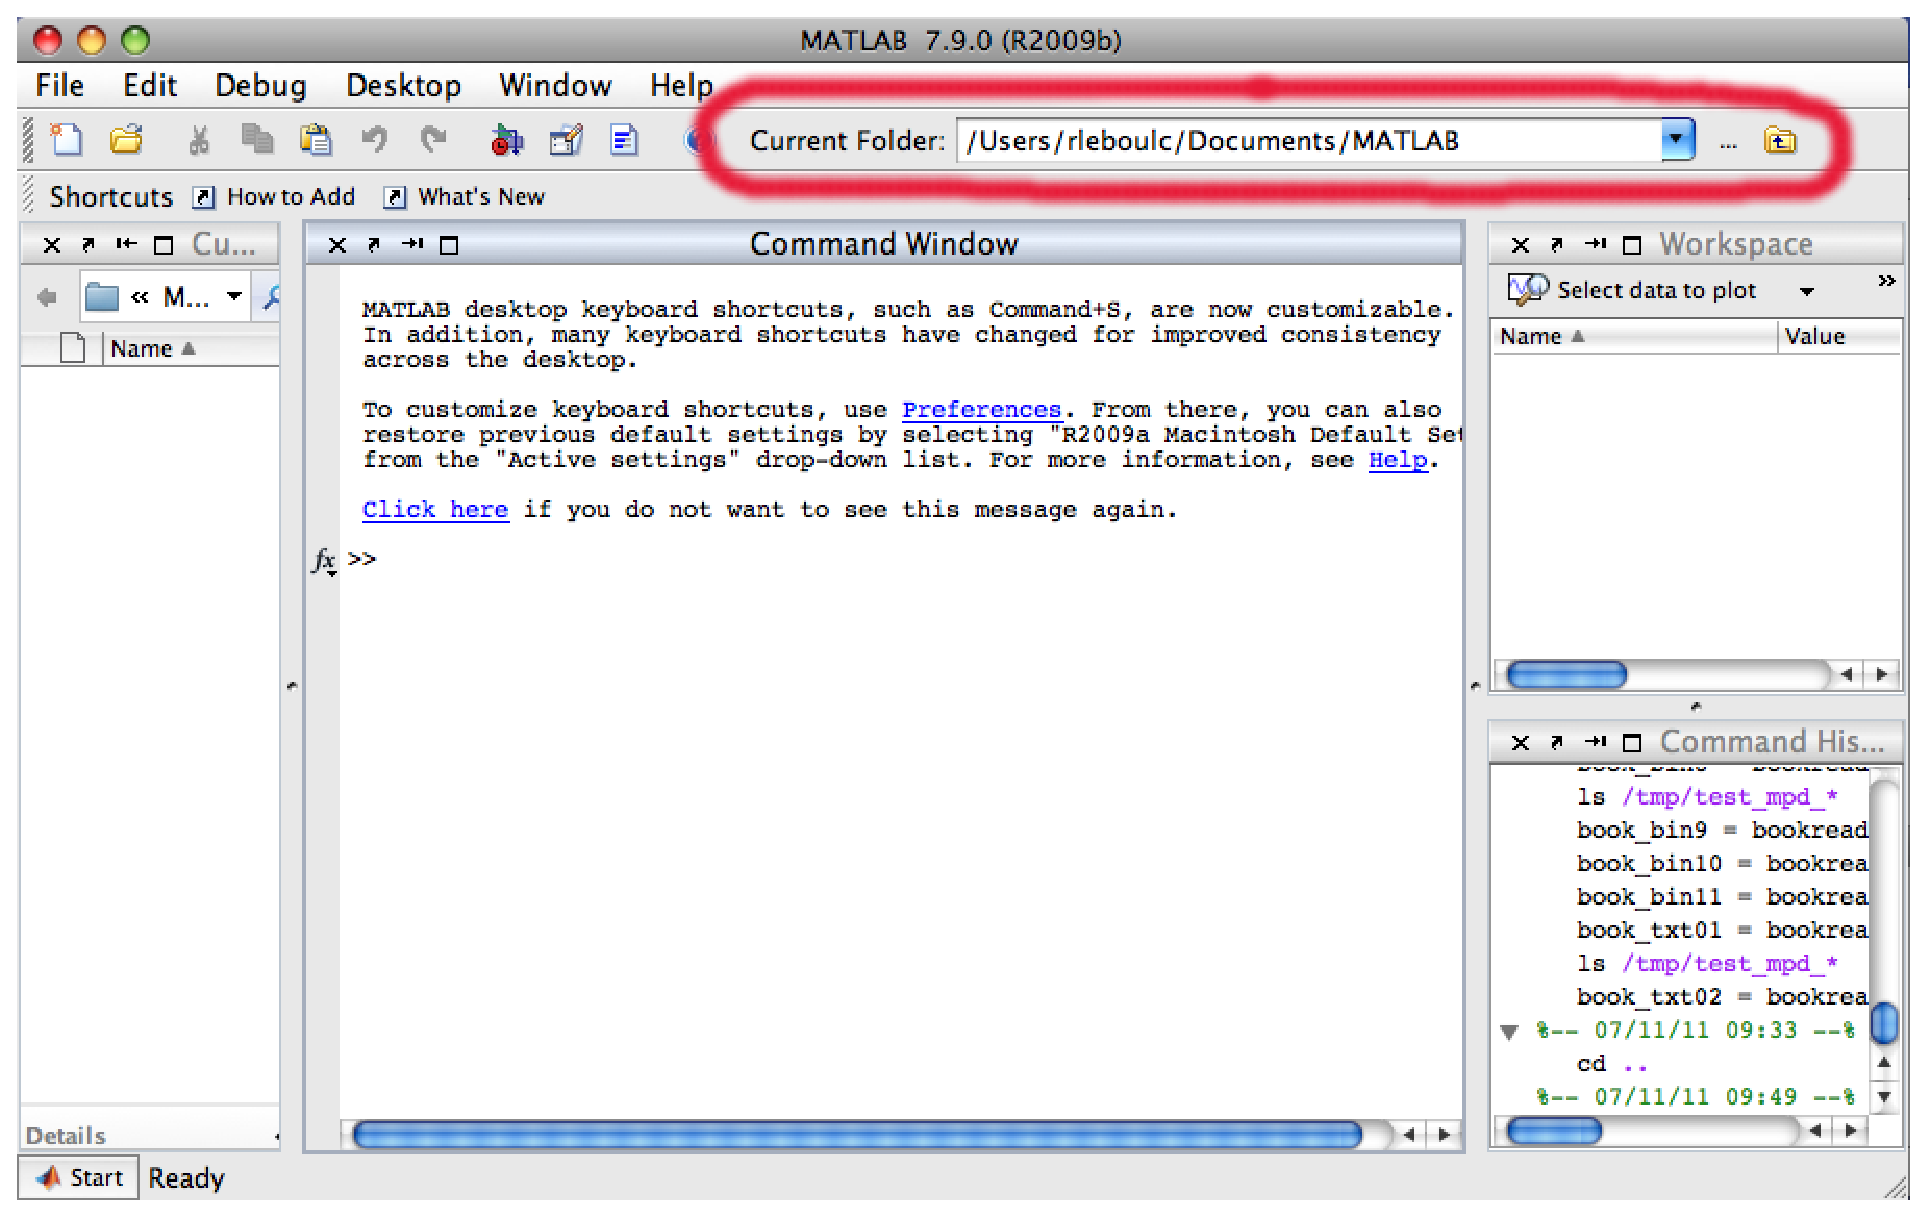
\includegraphics[width = 11cm, height=7cm]{Images/MatlabPathSelect.eps}
	\textit{\caption{\label{MatlabPathSelect} Description of Matlab selection path}}
\end{figure}

\clearpage

% Section 5.1.2 : Permanent path configuration

\subsection{Permanent path configuration}

When MATLAB is launched, it automatically executes the file ``matlabrc.m'' and, if it exists, ``startup.m''.
\begin{my_itemize}
	\item The file ``matlabrc.m'', under ``matlabroot/toolbox/local'', is reserved for MathWorks
	\item The file ``startup.m'' is for you to specify startup options
\end{my_itemize}

For example, you can modify the default search path or pre-define variables in your workspace. 
Use the following statements in a ``startup.m'' file to add the specified folder, ``path\_to\_MPTK/mptk/matlab'', to the search path.

\begin{tt}
	addpath(path\_to\_MPTK/mptk/matlab)
\end{tt}

\vspace {0.3 cm}

Place the ``startup.m'' file in the default or current startup folder, which is where MATLAB first looks for it.

%--------------------------------------------------------------
% Section 5.2 : Matlab book structure definition
%--------------------------------------------------------------
\section{Matlab book structure definition}

The book structure has been fully rewritten to fit ``bookedit'' needs and to allow fast operations on atoms. 
This structure is extensively used in ``GettingStarted.m'' so you can find many examples of processing a book with matlab.

\vspace{0.2 cm}

The original idea for the organization of the book is that atoms with the same sets of parameters (atoms 
of the same type: gabor, dirac, mdct, constant, ....) are gathered in atom sub structures for fast group processing.

\vspace{0.2 cm}

In order to further ease common atom manipulations, this idea has evolved into also grouping atoms of the same 
lengths. Now, in the book structure, there are as many ``atom'' as [atoms type*length]. This leads to ``book.atom'' 
structures rather close to the different ``blocks'' in the MP\_dictionary definition.

\vspace{0.2 cm}

\underline{The matlab `book' structure contains the following fields:}
\begin{my_itemize}
	\item format : Indicating the data format
	\item numAtoms : Number of atoms actually stored in the book
	\item numChans : number of channels of the atoms 
	\item numSamples : number of samples in each channel covered by the reconstructed book
	\item sampleRate : signal sample rate
	\item index: [ (4+numChans) x numAtoms matrix] : Index for reading/querying/sorting atoms with their occurrence in book\newline
		1 : Atom number in book (1 to numAtoms)\newline
		2 : Atom type\newline
		3 : Atom number in atom(type) structure\newline
		4 : Atom selected or not (used for saving part of a book)\newline
		4+channel : Atom position for channel 'channel' (1 to numChans)\newline
	\item atom:  [1 x Ntype struct]
	\begin{my_itemize}
		\item type : string
		\item params: structure of atoms parameters arrays, whose field are type dependent
	\end{my_itemize}
\end{my_itemize}

%--------------------------------------------------------------
%--------------------------------------------------------------
% Section 6 : List of Matlab functions
%--------------------------------------------------------------
%--------------------------------------------------------------
\chapter{List of Matlab functions \label{ListMatlabFunc}}
Some Matlab utilities are bundled with the distribution to help loading and visualizing books. 
They are automatically installed and can be found under mptk installation directory

\vspace{0.3 cm}

\noindent The stable included files are:
\begin{my_itemize}
	\item GettingStarted: A getting started example to use MPTK
	\item bookread: to load a binary book into Matlab
	\item bookwrite: to save a structured book into binary or txt format
	\item dictread: to read a dicitonary
	\item dictwrite: to write a dictionary
	\item mpdecomp: to decompose a signal into a book
	\item mprecons: to reconstruct a signal from a book
	\item sigread: reads and inport into matlab format an audio signal
	\item sigwrite: exports an audio signal from matlab to wav format
\end{my_itemize}

\noindent The non-stable included files are:
\begin{my_itemize}
	\item bookedit: to manually edit any book according to its structure
	\item bookplot: to plot a book in a spectrogram-like fashion
	\item bookover: to overlay a book plot on a STFT spectrogram
\end{my_itemize}

%--------------------------------------------------------------
% Section 6.1: Getting started
%--------------------------------------------------------------
\section{Getting Started}
\input{CommandUsage/getmptkinfo_Usage}
\clearpage

%--------------------------------------------------------------
% Section 6.2: bookread
%--------------------------------------------------------------
\section{bookread}
\input{CommandUsage/bookread_Usage}

%--------------------------------------------------------------
% Section 6.3: bookwrite
%--------------------------------------------------------------
\section{bookwrite}
\input{CommandUsage/bookwrite_Usage}

%--------------------------------------------------------------
% Section 6.4: bookedit
%--------------------------------------------------------------
\section{bookedit (see also chapter \ref{MatlabGUI})}
\input{CommandUsage/bookedit_Usage}
\clearpage

%--------------------------------------------------------------
% Section 6.5: bookplot
%--------------------------------------------------------------
\section{bookplot}
\input{CommandUsage/bookplot_Usage}

%--------------------------------------------------------------
% Section 6.6: bookover
%--------------------------------------------------------------
\section{bookover}
\input{CommandUsage/bookover_Usage}

%--------------------------------------------------------------
% Section 6.7: dictread
%--------------------------------------------------------------
\section{dictread}
\input{CommandUsage/dictread_Usage}

%--------------------------------------------------------------
% Section 6.8: dictwrite
%--------------------------------------------------------------
\section{dictwrite}
\input{CommandUsage/dictwrite_Usage}

%--------------------------------------------------------------
% Section 6.9: mpdecomp
%--------------------------------------------------------------
\section{mpdecomp}
\input{CommandUsage/mpdecomp_Usage}

%--------------------------------------------------------------
% Section 6.10: mprecons
%--------------------------------------------------------------
\section{mprecons}
\input{CommandUsage/mprecons_Usage}

%--------------------------------------------------------------
% Section 6.11: sigread
%--------------------------------------------------------------
\section{sigread}
\input{CommandUsage/sigread_Usage}

%--------------------------------------------------------------
% Section 6.12: sigwrite
%--------------------------------------------------------------
\section{sigwrite}
\input{CommandUsage/sigwrite_Usage}
\clearpage

%--------------------------------------------------------------
%--------------------------------------------------------------
% Section 7: Matlab bookedit GUI
%--------------------------------------------------------------
%--------------------------------------------------------------
\chapter{Matlab bookedit GUI \label{MatlabGUI}}

This GUI makes intensive use of function\_handles (denoted @functionName). The differents callbacks 
of the GUI are function handles which refer to sub functions. As a consequence, the code is divided in a large 
number of subfunctions. A tip to navigate inside the code is to select the function name, right-click and ``open selection''  
or F4 to jump to the sub-function.

The data (book info, selection info, figure handles and other variables) are organised in structure and are stored inside 
the figure. The data structure is loaded at the beginning of many functions and saved back at their end using the commands:
\begin{my_itemize}
	\item data = get(gcbf,`UserData'); \% load data
	\item set(gcbf,`UserData',data);   \% save data
\end{my_itemize}

%--------------------------------------------------------------
% Section 7.1: Interface startup
%--------------------------------------------------------------
\section{Interface startup}

The interface can be started under Matlab with �bookedit� command with different arguments:
\begin{my_itemize}
	\item No argument : At startup, a find file window asks the user for a valid MPTK book
	\item bookname: a string with a valid MPTK book. In this case the book is loaded at startup
\end{my_itemize}

%--------------------------------------------------------------
% Section 7.2: Overview and main functionalities
%--------------------------------------------------------------
\section{Overview and main functionalities}

Bookedit is a matlab tool to edit MTPK books issued from decomposition. It implements plotting tools, basic 
editing functions and audio transformations:
\begin{my_itemize}
	\item Plot atoms, toggle view per type and length
	\item Select atoms, Move, Cut or apply a gain on selected atoms
	\item Pitch Shifting and Time stretching of atoms
	\item Load / Save the modified MPTK book in native MPTK format
	\item Reconstruct and play the transformed/selected book
\end{my_itemize}

\clearpage

\noindent \underline{The following figure shows a snapshot of the interface:}

\begin{figure}[H]
	\centering
	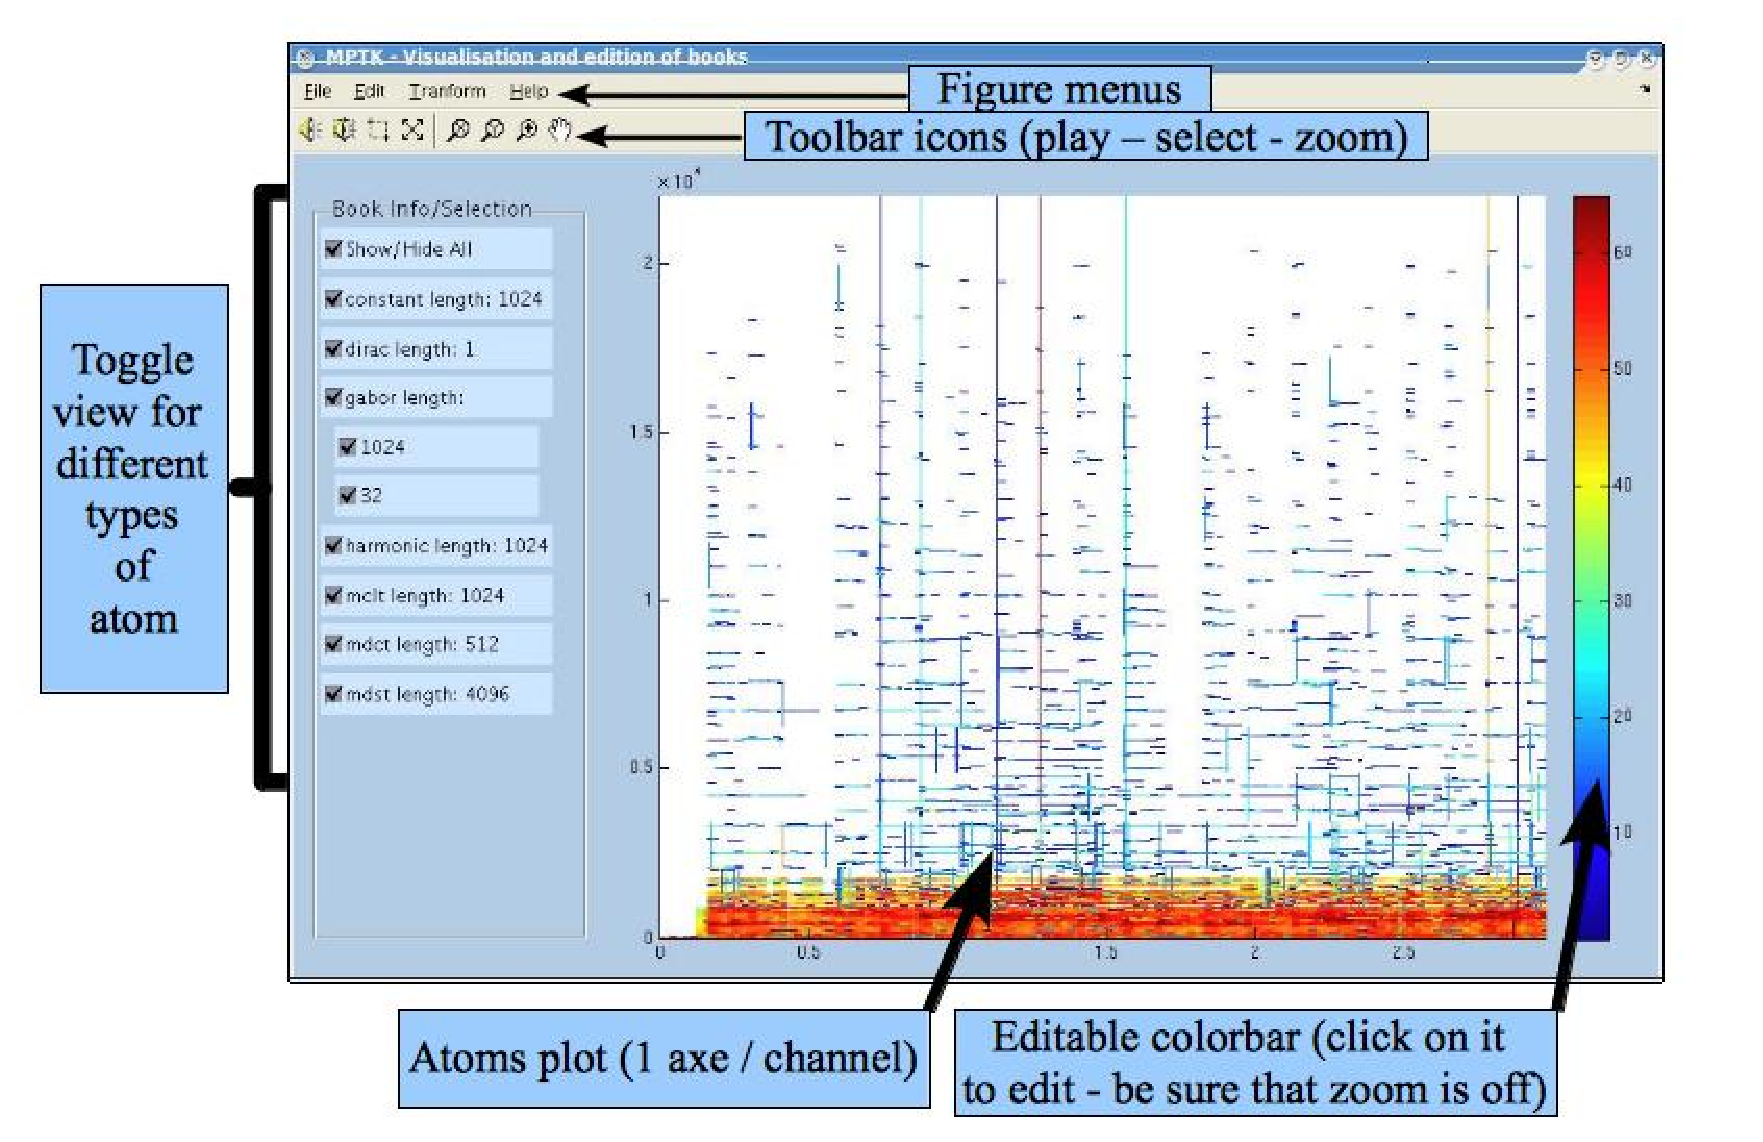
\includegraphics[width = 12cm, height=7cm]{Images/bookeditPage.eps}
	\textit{\caption{\label{bookeditPage} bookedit main page description}}
\end{figure}

%--------------------------------------------------------------
% Section 7.3: Toolbar functions
%--------------------------------------------------------------
\section{Toolbar functions}
\begin{figure}[H]
	\centering
	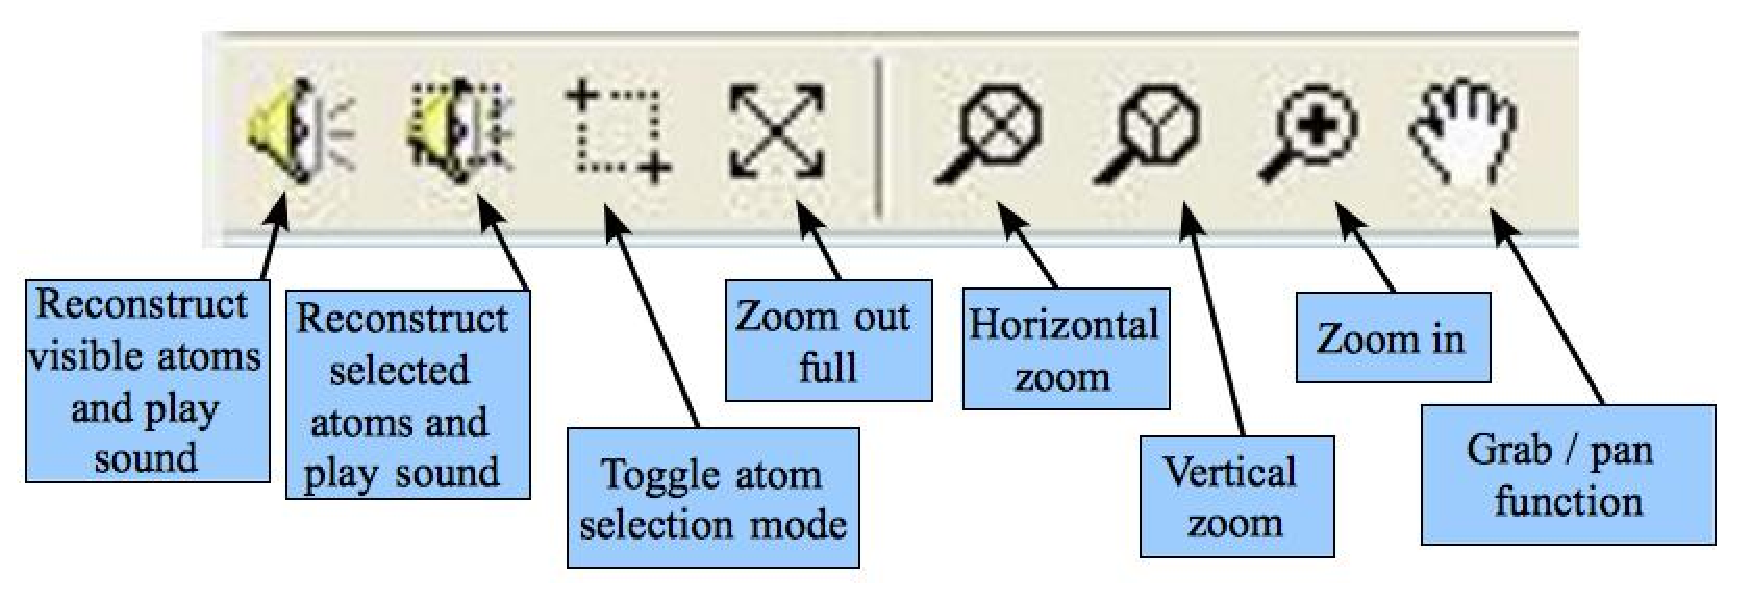
\includegraphics[width = 10cm, height=3cm]{Images/bookeditToolbar.eps}
	\textit{\caption{\label{bookeditToolbar} bookedit file toolbar description}}
\end{figure}

\noindent \textbf{Atom selection:} When the atom selection is toggled on, you can directly drag a rectangle in the 
plot to select an area. \newline
\noindent \textbf{Important note:} when a zoom function is active (icon grey) the colormap cannot be edited. 

%--------------------------------------------------------------
% Section 7.4: File Menu functions
%--------------------------------------------------------------
\section{File Menu functions}
\begin{figure}[H]
	\centering
	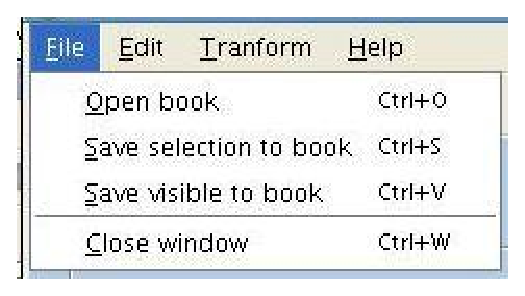
\includegraphics[width = 5cm, height=3cm]{Images/bookeditFileToolbar.eps}
	\textit{\caption{\label{bookeditFileToolbar} bookedit file toolbar description}}
\end{figure}

The `Edit' menu contains functions for editing the selected atoms.  It also has a `Refresh figure' 
usefull in case the GUI gets lost.

%--------------------------------------------------------------
% Section 7.5: Edit Menu functions
%--------------------------------------------------------------
\subsection{Edit Menu functions}
\begin{figure}[H]
	\centering
	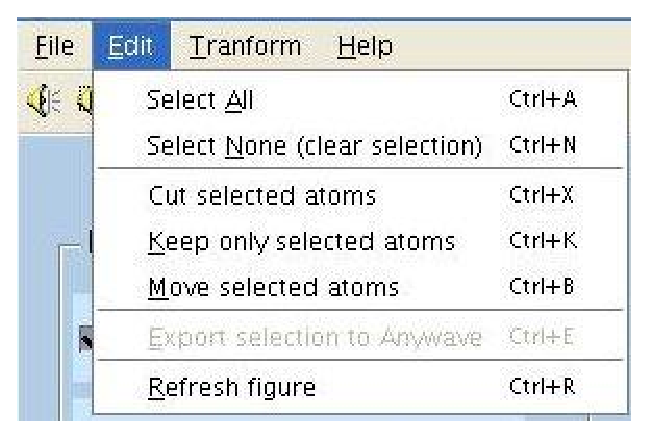
\includegraphics[width = 5cm, height=3cm]{Images/bookeditEditToolbar.eps}
	\textit{\caption{\label{bookeditEditToolbar} bookedit edit toolbar description}}
\end{figure}

The `File' menu contains functions for loading and saving a book. It possible to either save only the selected 
atoms or the visible part of the book.

%--------------------------------------------------------------
% Section 7.6: Transform Menu functions
%--------------------------------------------------------------
\subsection{Transform Menu functions}
\begin{figure}[H]
	\centering
	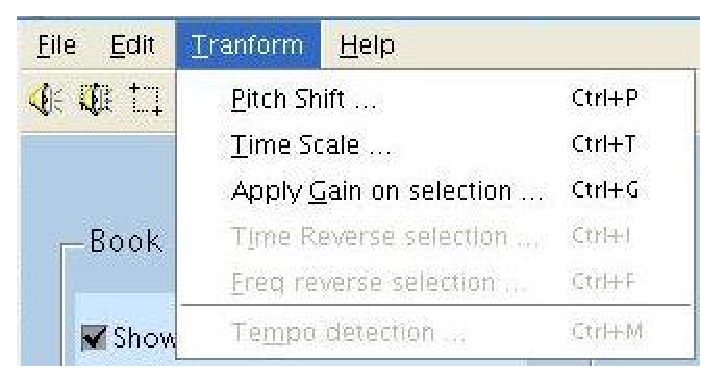
\includegraphics[width = 5cm, height=3cm]{Images/bookeditTransformToolbar.eps}
	\textit{\caption{\label{bookeditTransformToolbar} bookedit transform toolbar description}}
\end{figure}

The `Transform' menu contains functions for typical processing of audio signals. Some functions are not 
implemented and thus not accessible.

\clearpage

%--------------------------------------------------------------
%--------------------------------------------------------------
% Section 8: Testing if everything works
%--------------------------------------------------------------
%--------------------------------------------------------------

\chapter{List of Python functions \label{UsePythonFunc}}

The following sections list the commands available in pyMPTK.
See also Section \ref{GettingStartedPython} on getting started.

\section{`mptk' module: commands available}
\input{CommandUsage/Python_mptk_Usage}
\clearpage

\section{`mptkplot' module: commands available}
\input{CommandUsage/Python_mptkplot_Usage}
\clearpage

\chapter{Testing if everything works}
If you experiment some issues during the usage of MPTK, if you would like to ensure that the executables 
are working correctly, if you want to try new dictionaries, a series of tests are available on the source release.

%--------------------------------------------------------------
% Section 8.1 : Local tests using Ctest
%--------------------------------------------------------------
\section{Local tests using Ctest}

CTest is a testing tool distributed as a part of CMake. It can be used to automate updating, configuring, 
building, testing, performing memory checking, performing coverage, and submitting results to a CDash 
or Dart dashboard system.

You can run local tests on your machine using the command ``ctest'' if : 
\begin{my_itemize}
	\item MPTK has been successfully pre-compiled with cmake
	\item MPTK has been successfully compiled
	\item MPTK has been successfully installed
\end{my_itemize}

\begin{figure}[H]
	\centering
	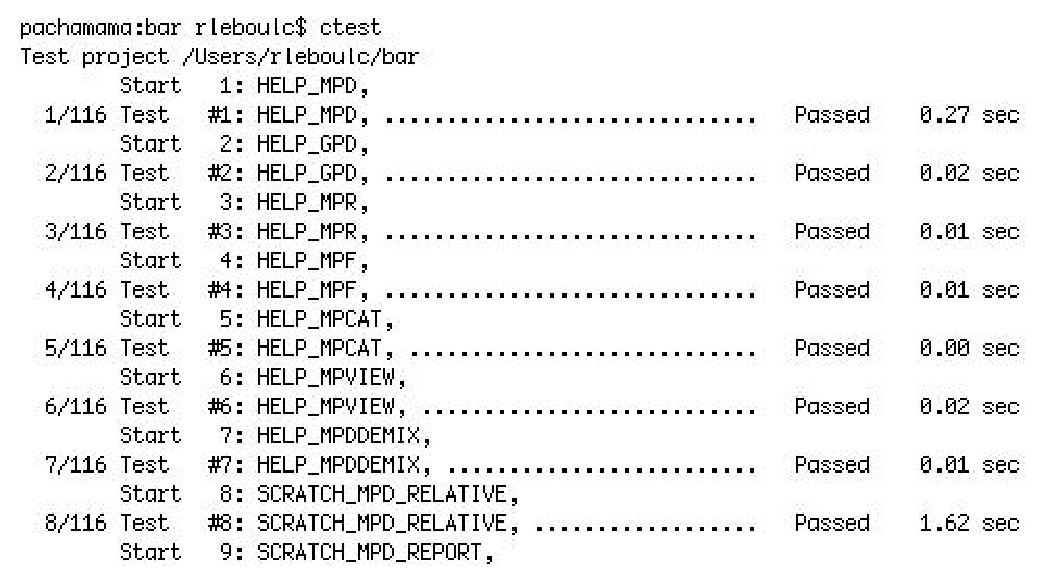
\includegraphics[width = 8cm, height=5cm]{Images/cTestReport.eps}
	\textit{\caption{\label{cTestReport} cTtest testing report description}}
\end{figure}

\clearpage

%--------------------------------------------------------------
%--------------------------------------------------------------
% Section 9: Format of the dicitionary files
%--------------------------------------------------------------
%--------------------------------------------------------------
\chapter{Format of the dictionary files \label{dict_format}}
The dictionary files use a XML syntax, with tags enclosed between
angle brackets. Strict XML compliance is now mandatory.
\footnote{Uh, that is, if a DTD get ready someday.}.

%--------------------------------------------------------------
% Section 9.1 : General rules
%--------------------------------------------------------------
\section{General rules \label{GenRules}}
A dictionary should include, in the following order:
\begin{my_enumerate}
	\item An optional XML declaration line;
	\item A mandatory dictionary opening tag;
	\item An optional library version tag;
	\item A list of blocks with their parameters (some mandatory, some admitting default values);
	\item A dictionary closing tag.
\end{my_enumerate}
Any text included after the dictionary closing tag will be ignored. Blank
spaces and line breaks are ignored. Any part of the file can be commented out
either by enclosing it between \verb+<!--+ and \verb+-->+ (XML style) 
The parser will send any text it can't match to stderr with a error message:
in the event of syntax errors in a dictionary, some dictionary
pieces will therefore show up in stderr.


\subsubsection{Valid tags}
\begin{scriptsize}
	\begin{alltt}
		\emph{<?xml version="1.0" encoding="ISO-8859-1"?>}
		          The XML declaration line.
		\emph{<dict>List of blocks</dict>}
		          The opening and closing tags for the dictionary. Anything coming after the </dict> tag 
		          will be ignored by the parser.
		\emph{<libVersion>blah</libVersion> [optional]}
		          The library version declaration. This is provided for backward compatibility if we ever 
		         change the dictionary syntax. If absent, the library version is taken to be the current one.
		\emph{<blockproperties name="PROPERTIES_NAME"> List of block parameters</blockproperties>}
		          The opening and closing tags for a block properties list.
		\emph{<block uses="PROPERTIES_NAME"> List of block parameters</block>}
		          The opening and closing tags for a block. The block will be construct using the list of 
		          parameters defined in PROPERTIES_NAME block properties.
		\emph{<block>List of block parameters</block>}
		          The opening and closing tags for a block. the list of block parameters should contains all 
		          the mandatories parameters for this type of block
		\emph{<param name="NAME" value="VALUE"/>}
		          A block parameter. The NAME and corresponding VALUE value in string. The parameter 
		          value is set to the corresponding type when the dictionary file is parsed. Note that when 
		          using the <block uses="PROPERTIES_NAME">List of block parameters </block> syntax. 
		          The block parameters defined in the block list override the parameters from 
		          PROPERTIES_NAME block properties.	
	\end{alltt}
\end{scriptsize}

\clearpage

\noindent The parameters list for block types (\textbf{G}abor, \textbf{H}armonic, \textbf{C}hirp, \textbf{A}nywave, \textbf{C}onsTant, \textbf{N}yquist):
\begin{my_itemize}
	\item {\tt windowLen (G,H,C,CT,N)} 
		\subitem Unsigned long int value: The atom length (i.e., the window length in the STFT)
	\item {\tt windowShift (G,H,C,A,CT,N)}
		\subitem Unsigned long int value: The atom shift (i.e., the window shift in the STFT)
	\item {\tt windowRate (G,H,C)}
		\subitem Double value between 0 and 1: An other way to specify the window shift, as a proportion 
		of the {\tt windowLen}.  If both are present, {\tt windowShift} has precedence over {\tt windowRate}
	\item {\tt fftSize (G,H,C)}
		\subitem Unsigned long value: The frequency resolution in terms of FFT size. It has to be greater 
		or equal to {\tt windowLen} if {\tt windowLen} is even, or $\geq$\verb2(windowLen+1)2 if \verb+windowLen+ 
		is odd. If absent, defaults to \verb+windowLen+ (or \verb2windowLen+12).
	\item  {\tt blockOffset (G,H,C,CT,N)} 
		\subitem Unsigned long value: the block Offset, (i.e. the position of the first frame
		If absent, defaults to 0
	\item {\tt windowtype (G,H,C,CT,N)}
		\subitem The window specification to be included among the block parameters
    	\item {\tt windowopt (G,H,C,CT,N)} 
		\subitem The optional parameter for window type parameter :
		\begin{my_itemize}
			\item Used for:  hamgen, gauss, exponential
			\item Not used for:  rectangle, triangle, cosine, hanning, hamming, blackman, flattop, fof
		\end{my_itemize}
		The meaning of the optional parameter varies according to the window type
	\item {\tt f0Min (H)} 
		\subitem Double value: minimum frequency (in Hz) from which the fundamental frequency 
		of the harmonic atoms is searched. Defaults to the first non-null FFT frequency
	\item {\tt f0Max (H)} 
		\subitem Double value: maximum frequency (in Hz) at which the fundamental frequency 
		of the harmonic atoms is searched. Defaults to the Nyquist frequency of the considered signal
	\item {\tt numPartials (H)} 
		\subitem Unsigned int value: number of partials considered when tracking the harmonic atoms
	\item {\tt numFitPoints (C)} 
		\subitem (EXPERIMENTAL) Unsigned int value: number of polynomial fitting points considered 
		for the chirp optimization algorithm. Defaults to 1.
	\item {\tt numIter (C)} 
		\subitem (EXPERIMENTAL) Unsigned int value: number of iterations considered for the chirp 
		optimization algorithm. Defaults to 1.
	\item {\tt chirpRateThreshold (C)} 
		\subitem (EXPERIMENTAL) Double value: maximum chirp-rate considered for the chirp 
		optimization algorithm. Defaults to 0.5e-5.
	\item {\tt checkUnchirped (C)} 
		\subitem (EXPERIMENTAL) Unsigned int value: 0 or 1, whether to check the chirped against the un-chirped 
		atom during the optimization (if so, may return un-chirped in preference if it shows better correlation).
		This can help to ensure stability, but it may tend to select unchirped atoms more than desired.
		Defaults to 1.
	\item {\tt tableFileName (A)} 
		\subitem String: filename of the table containing the waveforms (ex: /udd/toto/table.bin ). 
		Note that there is no {"} around the string.
\end{my_itemize}

\noindent \emph{Note :} The {\tt dirac} blocks don't need any parameter (they just match signal samples).

\clearpage

\subsubsection{Example}
\begin{tiny}
	\begin{alltt}
	          <?xml version="1.0" encoding="ISO-8859-1"?>                      \emph{\textcolor{cyan}{:The optional XML declaration line.}}
	          <dict>                                                           \emph{\textcolor{cyan}{:The dictionary opening tag.}}
	               <libVersion>0.2</libVersion>                           \emph{\textcolor{cyan}{:The optional library version.}}
	               <blockproperties name="GAUSS-WINDOW">	                  \emph{\textcolor{cyan}{:A new block properties.}}
	                         <param name="windowtype" value="gauss"/>
	                         <param name="windowopt" value="0.02"/>       \emph{\textcolor{cyan}{:Gauss windows need a parameter.}}
	               </blockproperties>
	               <block uses="GAUSS-WINDOW">                            \emph{\textcolor{cyan}{:New block using GAUSS-WINDOW.}} \emph
	                         <param name="type" value="gabor"/>
	                         <param name="windowLen" value="32"/>
	                         <param name="windowShift" value="32"/>
	                         <param name="fftSize" value="32"/>
	               </block>
	               <block>
	                         <param name="type" value="anywave"/>         \emph{\textcolor{cyan}{:An anywave block.}}
	                         <param name="tableFileName" value="/udd/toto/table.xml"/>
	                         <param name="windowShift" value="1"/>
	               </block>
	               <block>
	                         <param name="type" value="dirac"/>           \emph{\textcolor{cyan}{:A dirac block.}}
	               </block>
	               <block>
	                         <param name="type" value="constant"/>        \emph{\textcolor{cyan}{:A constant block.}}
	                         <param name="windowLen" value="512"/>
	                         <param name="windowShift" value="32"/>
	               </block>
	               <block>
	                         <param name="type" value="nyquist"/>         \emph{\textcolor{cyan}{:A nyquist block.}}
	                         <param name="windowLen" value="512"/>
	                         <param name="windowShift" value="32"/>
	               </block>
	          </dict>
	\end{alltt}
\end{tiny}

%--------------------------------------------------------------
% Section 9.2 : Anywave table
%--------------------------------------------------------------
\section{Anywave table}

Waveforms need have been loaded before using anywave atoms. That's the
difference between parametric atoms, such as Dirac, Gabor, ... and anywave
atoms. Therefore, a different syntax has to be employed. In the dictionary
file, the anywave block points to a ``anywave table definition file''
(/udd/toto/table.bin in the example). This file has a XML syntax, to give all
the parameters of the waveforms, and points to a binary ``anywave table data
file'', that gives the data (/udd/toto/table\_data.bin in the example).

Note that one table corresponds to one atom length, and one number of channels.
To use several atom lengths, create several anywave tables, and define
several ``anywave'' blocks.

\subsubsection{Valid tags}
\begin{scriptsize}
	\begin{alltt}
		\emph{<?xml version="1.0" encoding="ISO-8859-1"?>}
		     The XML declaration line.
		\emph{<dict>List of blocks</dict>}
		     The opening and closing tags for the dictionary. Anything coming after the </dict> tag 
		     will be ignored by the parser.
		\emph{<libVersion>blah</libVersion> [optional]}
		     The library version declaration. This is provided for backward compatibility if we ever 
		     change the dictionary syntax. If absent, the library version is taken to be the current one.
		\emph{<par type="NAME" value="VALUE"/>}
		     A table parameter. The NAME and corresponding VALUE value in string. The parameter 
		     value is set to the corresponding type when the table file is parsed. The NAME and 
		     corresponding VALUE types are given below:	
		          - {\tt numChans} (Unsigned short int): The number of channels of the atoms
		          - {\tt filterLen} (Unsigned long int): The length of the anywave waveforms in the table
		          - {\tt numFilters} (Unsigned long int): The number of anywave waveforms in the table
		          - {\tt data} (String): Name of the file containing the waveforms
	\end{alltt}
\end{scriptsize}

The ``anywave table data file'' is binary, and built as follows: all the
waveforms are written in double type, one after the other, and for each, one
channel after the other. The following scheme is for two channels and four
waveforms: {\center |w1c1|w1c2|w2c1|w2c2|w3c1|w3c2|w4c1|w4c2| }

\subsubsection{Example of an anywave table}
\begin{tiny}
	\begin{alltt}
		<?xml version="1.0" encoding="ISO-8859-1" ?>                         \emph{\textcolor{cyan}{:The optional XML declaration line.}}
		<dict>
		     <libVersion>0.6.0</libVersion>                             \emph{\textcolor{cyan}{:The optional library version.}}
		     <block>
		          <param name="blockOffset" value="" />
		          <param name="data" value="+HxVeGKDh7946h9..." /> \emph{\textcolor{cyan}{:The binary datas encoded with base64 (text format)}}
		          <param name="filterLen" value="128" />
		          <param name="numChans" value="1" />
		          <param name="numFilters" value="4" />
		          <param name="windowShift" value="1" />
		     </block>
		</dict>
	\end{alltt}
\end{tiny}

%--------------------------------------------------------------
% Section 9.3 : MDCT/MDST/MCLT
%--------------------------------------------------------------
\section{MDCT/MDST/MCLT}

\subsubsection{Definition}
The Modified Discrete Cosine Transform (MDCT) and the Modified Discrete Sine Transform (MDST) are two 
orthogonal transforms based on local cosine functions. The Modulated Complex Lapped Transform (MCLT) 
is the complex extension such as $MCLT=MDCT+i*MDST$. The atoms corresponding to the MCLT of a signal 
of length $N=PL$ and a window length of $2L$, are defined as:

\begin{equation}
	x_{p,k}(n) = w(n-pL) exp \left[ i \frac{\pi}{L} \left( (n-pL) + \frac{1}{2} + \frac{L}{2} \right) \left( k + \frac{1}{2} \right) \right]
\end{equation} 
with $n=0,..,N-1$, $k=0,..,L-1$ and $p=0,..,P-1$. $w$ is a window which is complementary in energy i.e. it verifies $w^2 (n) + w^2 (n+L) = 1, n=0,..,L-1$.

The atoms corresponding to the MDCT are defined as the real part of the previous formula and the atoms corresponding 
to the MDST the imaginary part of the previous formula. We also define a generalized MDCT/MDST/MCLT where the window 
shift, the window shape and the fft size are not constraint by the orthogonality property. The corresponding atoms for a signal 
of length $N=PS$, a window length of $2L$, a window shift of $S$, a fft size of $Nfft$ and a window $w$, are defined as:
\begin{eqnarray}
x_{p,k}(n) = w(n-pS) exp \left[ i \frac{2\pi}{Nfft} \left( (n-pS) + \frac{1}{2} + \frac{L}{2} \right) \left( k + \frac{1}{2} \right) \right] \mbox{ if } Nfft=2L \\
x_{p,k}(n) = w(n-pS) exp \left[ i \frac{2\pi}{Nfft} \left( (n-pS) + \frac{1}{2} + \frac{L}{2} \right) \left( k  \right) \right] \mbox{ if }Nfft=2mL
\end{eqnarray}
with $n=0,..,N-1$, $k=0,..,Nfft/2-1$, $p=0,..,P-1$ and m is even with $m>=2$.

\subsubsection{Valid tags}
\begin{scriptsize}
	\begin{alltt}
	\emph{<?xml version="1.0" encoding="ISO-8859-1"?> [optional]}
	     The XML declaration line.
	\emph{<libVersion>blah</libVersion> [optional]}
	     The library version declaration. This is provided for backward compatibility if we ever 
	     change the dictionary syntax. If absent, the library version is taken to be the current one.
	\emph{<dict>List of blocks</dict>}
	     The opening and closing tags for the dictionary. Anything coming after the </dict> tag 
	     will be ignored by the parser.
	\emph{<par type="NAME" value="VALUE"/>}
	     A table parameter. The NAME and corresponding VALUE value in string. The parameter
	     value is set to the corresponding type when the table parameter file is parsed. The NAME 
	     and corresponding VALUE types are given below:
	          - windowLen (Unsigned long int): The atom length (window length). It has to be even
	          - windowShift (Unsigned long int): The atom shift (window shift)
	          - windowRate (Double between 0.0 and 1.0:): An alternate way to spe-cify the window 
	            shift, as a proportion of the windowLen. If both are present, windowShift has precedence 
	            over windowRate
	          - fftSize (Unsigned long): The frequency resolution in terms of FFT size. It has to be equal
	            to windowLen or a multiple of 2*windowLen
	          - blockOffset (Unsigned long): The block Offset (position of the first frame). If absent, defaults to 0
	          - windowtype (Unsigned char): The window specification to be included among the block parameters
	          - windowopt (Double): The optional parameter for window type:
	               * Used: hamgen, gauss, exponential, kbd
	               * Not used: rectangle, triangle, cosine, hanning, hamming, blackman, flattop, fof
	\end{alltt}
 \end{scriptsize}
   

A default MDCT/MDST/MCLT block is defined using 2 parameters, the window length and the window type. The window type must be \verb+rectangle+, \verb+cosine+ or \verb+kbd+. 

An example of a MDCT dictionnary is:
\tiny\begin{verbatim}
<?xml version="1.0" encoding="ISO-8859-1"?>
        <dict>
        <libVersion>0.2</libVersion>
                <block>
                        <param name="type" value="mdct"/>
                        <param name="windowLen" value="2048"/>
                        <param name="windowtype" value="kbd"/>
                        <param name="windowopt" value="5"/>
                </block>
        </dict>
\end{verbatim}\normalsize

An example of a generalized MCLT dictionnary is:
\tiny\begin{verbatim}
<?xml version="1.0" encoding="ISO-8859-1"?>
        <dict>
        <libVersion>0.2</libVersion>
                <block>
                        <param name="type" value="mdct"/>
                        <param name="windowLen" value="2048"/>
                        <param name="fftSize" value="4096"/>
                        <param name="windowtype" value="cosine"/>
                        <param name="windowopt" value="0"/>
                </block>
        </dict>
\end{verbatim}\normalsize

%--------------------------------------------------------------
%--------------------------------------------------------------
% Section 10: Format of the book files
%--------------------------------------------------------------
%--------------------------------------------------------------
\chapter{Format of the book files \label{book_format}}

The book files can be used either as a binary or XML files. They are divided into 
two different parts. The first part (xml style) includes all the different dictionaries used during 
the decomposition. The second part (xml or binary style) represents the differents atom
founded during the decomposition.

%--------------------------------------------------------------
% Section 10.1 : General rules
%--------------------------------------------------------------
\section{General rules}
A book should include, in the following order:
\begin{my_enumerate}
	\item An optional XML declaration line;
	\item A dictionary XML structure (see section \ref{GenRules})
	\item A `bin' or `txt' string refering to the following book structure
	\item A book opening tag (including mandatory parameters)
	\item A book closing tag.
\end{my_enumerate}

Any text included after the book closing tag will be ignored. Blank
spaces and line breaks are ignored. Any part of the file can be commented out
either by enclosing it between \verb+<!--+ and \verb+-->+ (XML style) 
The parser will send any text it can't match to stderr with a error message:
in the event of syntax errors in a dictionary, some dictionary
pieces will therefore show up in stderr.

% Section 10.1.1 : Valid tags

\subsubsection{Valid tags}
\begin{scriptsize}
	\begin{alltt}
		\emph{<?xml version="1.0" encoding="ISO-8859-1"?>}
		          The XML declaration line.
		\emph{<dict>List of blocks</dict>}
		          The opening and closing tags for the dictionary. Anything coming after the </dict> tag 
		          will be ignored by the parser.
		\emph{<libVersion>blah</libVersion> [optional]}
		          The library version declaration. This is provided for backward compatibility if we ever 
		         change the dictionary syntax. If absent, the library version is taken to be the current one.
		\emph{<blockproperties name="PROPERTIES_NAME"> List of block parameters</blockproperties>}
		          The opening and closing tags for a block properties list.
		\emph{<block uses="PROPERTIES_NAME"> List of block parameters</block>}
		          The opening and closing tags for a block. The block will be construct using the list of 
		          parameters defined in PROPERTIES_NAME block properties.
		\emph{<block>List of block parameters</block>}
		          The opening and closing tags for a block. the list of block parameters should contains all 
		          the mandatories parameters for this type of block
		\emph{<param name="NAME" value="VALUE"/>}
		          A block parameter. The NAME and corresponding VALUE value in string. The parameter 
		          value is set to the corresponding type when the dictionary file is parsed. Note that when 
		          using the <block uses="PROPERTIES_NAME">List of block parameters </block> syntax. 
		          The block parameters defined in the block list override the parameters from 
		          PROPERTIES_NAME block properties.	
		\emph{`bin' or `txt' string}
		          A string describing if the following book structure is in binary format or in text (XML) format
		\emph{<book nAtom=``x'' numChans=``x'' numSamples=``x'' sampleRate="x" libVersion="x.x.x">}
		          The book opening tag. It includes the number of atoms founded, the number of channels of 
		          the signal, the number of samples and the sample rate asked by the user and the library version
		\emph{xwA&=<?#_8zk*�?gabor}
                            An atom datas. It includes the binary datas (``xwA...'') and the name of the type of the atom used
		\emph{</book>}
                            The book closing tag.
	\end{alltt}
\end{scriptsize}

%%%%%%%%%
\appendix
%%%%%%%%%
\cleardoublepage
%%%%%%%%%

%--------------------------------------------------------------
%--------------------------------------------------------------
%--------------------------------------------------------------
% Section A : Gettting libsndfile
%--------------------------------------------------------------
%--------------------------------------------------------------
%--------------------------------------------------------------
\chapter{Getting libsndfile \label{GetLibsndfile}}

Libsndfile is a C library for reading and writing files containing sampled sound (such as MS 
Windows WAV and the Apple/SGI AIFF format) through one standard library interface. It is released 
in source code format under the Gnu Lesser General Public License. 

This library can be downloaded either through the web (for example via Mega-Nerd website) or in 
the ``relased files'' section of the MPTK Gforge:
\begin{my_itemize}
	\item http://www.mega-nerd.com/libsndfile/
	\item http://mptk.gforge.inria.fr/
\end{my_itemize}

Install this package on your computer using the instructions given on this web site will be easy an 
will yield the following sequence of commands after unzipping the package: \newline
\textcolor[rgb]{0.4,0.4,0.4}{./configure [options]} \newline
\textcolor[rgb]{0.4,0.4,0.4}{make} \newline
\textcolor[rgb]{0.4,0.4,0.4}{make install} \newline

%--------------------------------------------------------------
%--------------------------------------------------------------
%--------------------------------------------------------------
% Section B : Gettting fftw
%--------------------------------------------------------------
%--------------------------------------------------------------
%--------------------------------------------------------------
 \chapter{Getting fftw \label{GetFftw}}

FFTW is a C subroutine library for computing the discrete Fourier transform (DFT) in one or more 
dimensions, of arbitrary input size, and of both real and complex data (as well as of even/odd data, 
i.e. the discrete cosine/sine transforms or DCT/DST). 

This library can be downloaded either through the web or in the ``relased file''� section of the MPTK Gforge:
\begin{my_itemize}
	\item http://www.fftw.org/install/windows.html
	\item http://mptk.gforge.inria.fr/
\end{my_itemize}

Install this package on your computer using the instructions given on this web site will be easy an will 
yield the following sequence of commands after unzipping the package: \newline
\textcolor[rgb]{0.4,0.4,0.4}{./configure [options]} \newline
\textcolor[rgb]{0.4,0.4,0.4}{make} \newline
\textcolor[rgb]{0.4,0.4,0.4}{make install} \newline

%--------------------------------------------------------------
%--------------------------------------------------------------
%--------------------------------------------------------------
% Section C : References
%--------------------------------------------------------------
%--------------------------------------------------------------
%--------------------------------------------------------------
\chapter{References}
\section{Algorithmic aspects} For more information about the algorithmic
aspects of the Matching Pursuit algorithm, see: \newline \cite{Zhang93},
\cite{MZ93}, \cite{PRK93}, \cite{Davis94}, \cite{Bergeaud},
\cite{BM96}, \cite{HRP}, \cite{HRMP1}, \cite{HRMP2}, \cite{DMA97},
\cite{goodwin99:_match}, \cite{MaThese}, \cite{Grib2001}, \linebreak
\cite{Grib2002a}, \cite{gribonval03:_harmon_decom_audio_signal_match_pursuit},
\cite{SPIE03:GribA}, \cite{IC06MPTK}.

\section{Theoretic aspects} For more information about the theoretic aspects
of the Matching Pursuit algorithm, see: \newline
\cite{Grib2001b}, \cite{GN2001}, \cite{Grib2001c}, \cite{ICIP03:GN},
\cite{gribonval03:_spars}, \cite{IRISA03:GV}, \cite{gribonval03:_highl},
\cite{GribFig}.

\section{Experimental results and applications} Examples of experimental and
applicative results obtained with MPTK can be found in: \newline
\cite{WASPAA05}, \cite{LESAGE_ICA06}.


%%%%%%%%%
{\bibliographystyle{apalike}
\bibliography{biblio_MP}}

\end{document}


